\documentclass[a4paper,12pt]{article}
\usepackage[utf8]{inputenc}
\usepackage{amsfonts,amstext}
\usepackage{amsmath,amssymb}
\usepackage{amsthm}
% \usepackage{german}
\usepackage[ngerman]{babel}
\usepackage{fullpage}
\usepackage[a4paper,margin=3cm]{geometry}
\usepackage{hyperref}
\usepackage{listings}
\usepackage[usenames,dvipsnames]{xcolor}
% \usepackage[noend]{algpseudocode}
% \usepackage{algorithm}
\usepackage{fancyhdr}
\usepackage{lastpage}
\usepackage{graphicx}
\usepackage{float}
\usepackage{bookmark}
\usepackage[parfill]{parskip} % https://tex.stackexchange.com/questions/74170/have-new-line-between-paragraphs-no-indentation#74173



% https://www.overleaf.com/learn/latex/Theorems_and_proofs
% https://www.overleaf.com/learn/latex/Theorems_and_proofs#Reference_guide
\theoremstyle{definition}
\newtheorem*{example}{Beispiel}
\newtheorem{definition}{Definition}[section]

\theoremstyle{plain}
\newtheorem{theorem}{Satz}[section]
\newtheorem{lemma}[definition]{Lemma}

\theoremstyle{remark}
\newtheorem*{remark}{Bemerkung}
\newtheorem*{notation}{Notation}
\newtheorem*{question}{Frage}


% Defining \lsem and \rsem without using MnSymbol because it causes other symbols (like \in) to look different
\newcommand{\lsem}{\mathrm{[}\kern-.14em\mathrm{[}}
\newcommand{\rsem}{\mathrm{]}\kern-.14em\mathrm{]}}
\newcommand{\zb}{z.\,B.}
\renewcommand{\dh}{d.\,h.}
\newcommand{\floor}[1]{\left\lfloor{#1}\right\rfloor}
\newcommand{\ceil}[1]{\left\lceil{#1}\right\rceil}
\newcommand{\half}[1]{\frac{#1}{2}}
\newcommand{\sem}[1]{S\lsem#1\rsem}
\newcommand{\Bsem}[1]{\mathcal{B}\lsem#1\rsem}
\newcommand{\Asem}[1]{\mathcal{A}\lsem#1\rsem}
\newcommand{\Nsem}[1]{\mathcal{N}\lsem#1\rsem}
\newcommand{\Ssem}[1]{\mathcal{S}\lsem#1\rsem}
% Zustandsüberführungsrelation natürliche Semantik
\newcommand{\strans}[3]{\langle #1, #2 \rangle \to #3}
\newcommand{\stranssos}[3]{\langle #1, #2 \rangle \Rightarrow #3}
% Schlussregel natürliche Semantik
\newcommand{\infruleNs}[2][]{[\text{#2}_{\text{ns}}^{#1}]}
% Schlussregel strukturelle Semantik
\newcommand{\infruleSos}[2][]{[\text{#2}_{\text{sos}}^{#1}]}

\newcommand{\figref}[1]{Abbildung~\ref{#1}}
\newcommand{\secref}[1]{Abschnitt~\ref{#1}}
\newcommand{\defref}[1]{Definition~\ref{#1}}
\newcommand{\defrefshort}[1]{\text{D.}~\ref{#1}}  % for math mode

\DeclareMathOperator{\bits}{\{0,1\}}
\DeclareMathOperator{\AExp}{AExp}
\DeclareMathOperator{\BExp}{BExp}
\DeclareMathOperator{\Stm}{Stm}
\DeclareMathOperator{\Num}{Num}
\DeclareMathOperator{\Var}{Var}
\DeclareMathOperator{\State}{State}
\DeclareMathOperator{\A}{\mathcal{A}}
\DeclareMathOperator{\B}{\mathcal{B}}
\DeclareMathOperator{\N}{\mathcal{N}}
\DeclareMathOperator{\FV}{FV}
\DeclareMathOperator{\DV}{DV}
\DeclareMathOperator{\Env}{Env}
\DeclareMathOperator{\env}{env}
\DeclareMathOperator{\akt}{akt}
\DeclareMathOperator{\true}{w}
\DeclareMathOperator{\false}{f}

\renewcommand{\labelenumi}{(\alph{enumi})}


\definecolor{codegreen}{rgb}{0,0.6,0}
\definecolor{codegray}{rgb}{0.5,0.5,0.5}
\definecolor{codepurple}{rgb}{0.58,0,0.82}
\definecolor{backcolor}{rgb}{0.95,0.95,0.95}

\lstdefinestyle{mystyle}{
    backgroundcolor=\color{backcolor},
    commentstyle=\color{codegreen},
    keywordstyle=\color{magenta},
    numberstyle=\tiny\color{codegray},
    stringstyle=\color{codepurple},
    basicstyle=\ttfamily\small,
    breakatwhitespace=false,
    breaklines=true,
    captionpos=b,
    keepspaces=true,
    numbers=left,
    numbersep=6pt,
    showspaces=false,
    showstringspaces=false,
    showtabs=false,
    tabsize=2
}
\lstset{style=mystyle}
% \lstset{language=C}


\setlength{\headheight}{14.5pt}
\setlength{\headsep}{16pt}
\pagestyle{fancy}
\fancyhf{}
\renewcommand{\headrulewidth}{2pt}
\renewcommand{\footrulewidth}{1pt}
\lhead{\leftmark}
% \rhead{\rightmark}
\cfoot{Seite~\thepage~von~\pageref{LastPage}}



\begin{document}


\title{
    Semantik von Programmiersprachen \\[6pt]
    \large Vorlesung SoSe 2022 \\
    Wolfgang Mulzer
}
\author{Jim Neuendorf}
\maketitle
\begin{abstract}
    \noindent Diese Vorlesung vermittelt Techniken zur Formalisierung der Semantik (Be"-deu"-tungs"-inhalte) von Programmiersprachen. Zunächst werden unter"-schied"-liche Forma"-li"-sie"-rungs"-ansätze (die operationelle, denotationelle und axio"-ma"-ti"-sche Semantik) vorgestellt und diskutiert. Anschließend wird die mathe"-ma"-ti"-sche Theorie der semantischen Bereiche behandelt, die bei der deno"-tatio"-nel"-len Methode, Anwendung findet. Danach wird schrittweise eine umfassende, impe"-rative Programmiersprache entwickelt und die Semantik der einzelnen Sprach"-ele"-mente denotationell spezifiziert. Dabei wird die Fortsetzungstechnik (con"-tinua"-tion sem) systematisch erklärt und verwendet. Schließlich wird auf die Anwendung dieser Techniken eingegangen, insbesondere im Rahmen des Com"-piler"-baus und als Grundlage zur Entwicklung funktionaler Programmier"-spra"-chen.
\end{abstract}

\newpage
\tableofcontents

\hfill 29.04.

\section{Semantik}


Ziel: Finde eine mathematische Methode, um einem Programm eine \emph{Bedeutung} zuzuordnen.

Motivation:
\begin{itemize}
    \item Verifikation:
        \begin{itemize}
            \item Erfüllt mein Programm die Spezifikation (tut es das, was es soll)?
            \item Setzt der Übersetzer/Interpretierer die Spezifikation der Sprache korrekt um?
        \end{itemize}
     \item Programmumformung
        \begin{itemize}
            \item Haben zwei unterschiedliche Programme die gleiche Bedeutung?
            \item Optimierung
        \end{itemize}
    \item Programmanalyse
        \begin{itemize}
            \item Ist das Programm ``sicher'' (secure vs. safe)?
            \item Ist das Programm ``effizient''?
        \end{itemize}
\end{itemize}

\begin{definition}[Programmierparadigma]
    Programmierparadigma: \zb deklarativ (``Was?'') (funktional vs. logisch), imperativ (``Wie?''). In verschiedenen Paradigmen haben (potenziell) Programme verschiedene Bedeutungen.
\end{definition}

Wir konzentrieren uns auf \emph{imperative} Programmierung.

\begin{question}
    Was ist die ``mathematische Bedeutung'' eines imperativen Programms?
\end{question}

\begin{question}[folgend]
    Was ist ein imperatives Programm?
\end{question}



\begin{lstlisting}[language=Python, caption=Imperatives Programm]
x = 1
y = x + 2
x = y + 5
for ...
\end{lstlisting}
% => Es gibt einen Zustand (alles, was im Speicher steht). Diesen ändert man mit Zuweisung


\begin{lstlisting}[language=Haskell, caption=Funktionales Programm]
foo :: Int -> Int
foo 0 = 1
foo x = x + 1
foo 3
\end{lstlisting}
% => kein Zustand, sondern es gibt einen Ausdruck, der ausgewertet wird

Das zentrale Konzept der imperativen Programmierung ist der \emph{Zustand} (state). Der Zustand ist der Inhalt aller Speicherzellen und Register, die Position des Programm"-zählers und der Zustand der Eingabe-/Ausgabe-Geräte.

Ein imperatives Programm ist eine Folge von \emph{Anweisungen} (statement / instruction). Diese haben \emph{Wirkungen} (effects), welche den Zustand verändern (selbst \texttt{nop} ändert den Programmzähler und somit den Zustand). Darüber hinasu gibt es Neben"-wir"-kungen bzw. Seiteneffekte (side effects). Es gibt unterschiedliche Arten von Anwei"-sungen:
\begin{itemize}
    \item Zuweisungen (direkte Änderung des Zustandes)
    \item Kontrollfluss (Änderung des Programmzählers: Verzweigungen, Schleifen, Funk"-tions"-aufrufe bzw. Sprünge)
    \item Eingabe / Ausgabe
\end{itemize}

\section{Mathematische Formalisierung}

\begin{definition}[Zustand]
    Es gibt eine abzählbar unendliche Menge von Variablen $V = \{ x_1, x_2, \dots, y, z, \dots \}$ (Speicher ist begrenzt aber beliebig groß). Der Zustand ist eine (partielle) Funktion \[
    \sigma: V \to \mathbb{Z} \cup \{ \bot, \true, \false \}
    \]
    ($\bot$ bedeutet undefiniert, \dh{} eine Speicherzelle hat noch keinen Wert und die Funk"-tion gibt nichts aus).

    Die Teile des Zustandes ``Eingabe / Ausgabe'' ignorieren wir erst einmal, \dh{} die initiale Eingabe ist implizit durch den Wert der Variablen am Anfang. Der Programm"-zähler wird an anderer Stelle thematisiert.
\end{definition}

\begin{remark}
    Diese Definition dient als Beispiel, \dh{} in anderen Szenarien mit anderen Variablen außer Ganzzahlen und Boolesche Wert kann eine andere Definition sinnvoller sein.
\end{remark}

\begin{definition}[Imperatives Programm]
    Ein imperatives Programm ist eine Funktion auf der Menge alles Zustände. Jedem Startzustand wird ein Endzustand zugeordnet (wir ignorieren E/A).
\end{definition}

\begin{notation}
    Sei $\Pi \in \Sigma^*$ ein gültiges Programm (eine Zeichenkette). Wir bezeichnen mit
    \[
    \sem{\Pi} \in [State \to State]
    \]
    ($S$ ist die semantische Funktion) die Funktion, welche durch $\Pi$ definiert wird.
\end{notation}



\subsection{\texttt{while}-Sprache}\label{section:while}

\begin{definition}
    Wir verwenden in dieser Vorlesung eine einfache, turing-vollständi"-ge, imperative Programmiersprache als durchgängiges Beispiel namens \texttt{while}-\emph{Spra"-che}, die durch folgende kontextfreie Grammatik gegeben ist:
\end{definition}
\vspace*{-2em}
\begin{align*}
    A & \to \texttt{Zahl | Var | $A + A$ | $A * A$ | $A - A$} \\
    B & \to \texttt{true | false | $A = A$ | $A \leq A$ | $\neg B$ | $B \wedge B$} \\
    S & \to \texttt{Var := A | skip | S; S | if B then S else S | while B do S}
\end{align*}
\begin{remark}
    Es gibt die syntaktischen Kategorien ``arithmetischer Ausdruck'' ($A$), ``Boolescher Ausdruck'' ($B$) und ``Statement'' ($S$, Anweisung).
\end{remark}

\begin{example}
    \begin{align*}
        \Pi & = \texttt{x := z + 1} \\
        \Ssem{\texttt{x := z + 1}}(\underbrace{[x \mapsto 5, z \mapsto -4, a \mapsto 2]}_{\text{Startzustand}}) & = \underbrace{[x \mapsto -3, z \mapsto -4, a \mapsto 2]}_{\text{Endzustand}} \\
        \Ssem{\texttt{x := z + 3}}([x \mapsto 10, z \mapsto 12]) & = [x \mapsto 15, z \mapsto 12]
    \end{align*}
\end{example}

\fbox{Für diese Veranstaltung stellen wir uns die Frage: Wie komme ich von $\Pi$ zu $\sem{\Pi}$?}


Dafür gibt es drei Ansätze:
\begin{enumerate}
    \item axiomatische Semantik
    \item operationelle Semantik
    \item denotationelle Semantik
\end{enumerate}


\subsection{Axiomatische Semantik}

Wir verzichten auf die vollständige Spezifikation von $\sem{\cdot}$. Stattdessen arbeiten wir mit \emph{Zusicherungen} (Assertions), welche wesentliche Aspekte des Zustands zu einem gegebenen Zeitpunkt widerspiegeln.

Wir definieren ein logisches System, das Beziehungen zwischen Zuständen aufstellt (Vorbedingungen, Nachbedingungen). Das System muss $\sem{\cdot}$ verträglich sein.

Die Details sind Thema einer anderen Vorlesungen, \zb{} Hoare-Kalkül.

\begin{example}
    \[
    \underbrace{\{ x = n \wedge y = m \}}_{\text{Vorbedingung}} \quad \texttt{z := x; x := y; y := z} \quad \underbrace{\{ x = m \wedge y = n \}}_{\text{Nachbedingung}}
    \]
\end{example}



\subsection{Operationelle Semantik}

Definiere $\sem{\Pi}$ durch schrittweise Simulation der Ausführung von $\Pi$ (ein Interpretierer in mathematischer Form / Abstraktion).

Genauer gesagt bedeutet das: Wir definieren ein \emph{Transitionssystem}
\begin{align*}
    \langle \Pi, s \rangle & \Rightarrow \langle \Pi', s' \rangle \\
    \langle \Pi, s \rangle & \Rightarrow s'
\end{align*}
das die Ausführung von $\Pi$ auf Zustand $s$ darstellt.

\begin{example}
    \begin{align*}
        & \langle \texttt{z := x; x := y; y := z}, [x \mapsto 2, y \mapsto 3, z \mapsto 6] \rangle \\
        \Rightarrow \; & \langle \texttt{x := y; y := z}, [x \mapsto 2, y \mapsto 3, z \mapsto 2] \rangle \quad\quad \text{(1. Befehl ausgeführt)} \\
        \Rightarrow \; & \langle \texttt{y := z}, [x \mapsto 3, y \mapsto 3, z \mapsto 2] \rangle \\
        \Rightarrow \; & [x \mapsto 3, y \mapsto 2, z \mapsto 2] \quad\quad \text{(Endzustand)}
    \end{align*}
\end{example}



%%%%%%%%%%%%%%%%%%%%%%%%%%%%%%%%%%%%%%%%%%%%%%%%%%%%%%%%%%%%%%%%%%%%%
\newpage
\hfill 06.05.
%%%%%%%%%%%%%%%%%%%%%%%%%%%%%%%%%%%%%%%%%%%%%%%%%%%%%%%%%%%%%%%%%%%%%


\subsection{Denotationelle Semantik}

Definiere $\sem{\Pi}$ direkt als mathematische Funktion anhand der Syntax von $\Pi$, \zb{}
\begin{align*}
    \Ssem{\texttt{z := x; x := y; y := z}} & = \Ssem{\texttt{y := z}} \circ \Ssem{\texttt{x := y}} \circ \Ssem{\texttt{z := x}}
\end{align*}

Es wird also \zb{} die sequenzielle Ausführung von Anweisungen als Funktionskomposition übersetzt.

\begin{remark}[Problem]
    Wie kann man beispielsweise Schleifen darstellen (insbesondere \texttt{while})? Ein möglicher Ansatz sind Grenzwerte, aber das geht tiefer in die Analysis.
    Bei der operationellen Semantik wird die Schleife durch das Transitionssystem realisiert.
\end{remark}

\section{Operationelle Semantik}

Das Folgende bezieht sich auf die \texttt{while}-Sprache (siehe \secref{section:while}).

\begin{definition}
    $\AExp, \BExp, \Stm$: Mengen aller gültigen Ableitungen aus $A$, $B$ bzw. $S$ als Syntaxbaum. Der Ausdruck \texttt{5+7-2*8} lässt sich aus $A$ ableiten. Der entsprechende Syntaxbaum (siehe \figref{fig:syntaxbaum}) ist dann Teil von $\AExp$.
    \[
    a \in \AExp
    \]
    Mengen wie $\AExp$ bezeichnen wir als \textbf{syntaktische Kategorien}.

    \textbf{Zahl} ist eine ganze Zahl aus $\mathbb{Z}$. Die zugehörige syntaktische Kategorie ist $\Num$. Sie ist die Menge aller Zeichenketten, die ganze Zahlen darstellen.
    \begin{align*}
        \texttt{1234} & \in \Num \\
        1234 & \in \mathbb{Z}
    \end{align*}
    Beachte, dass eigentlich der Syntaxbaum von \texttt{1234} gemeint ist.

    $\Var$ sind Variablen, die nach Belieben vorhanden sind. Es sind abzählbar unendlich viele.
\end{definition}

\begin{figure}[H]
    \centering
    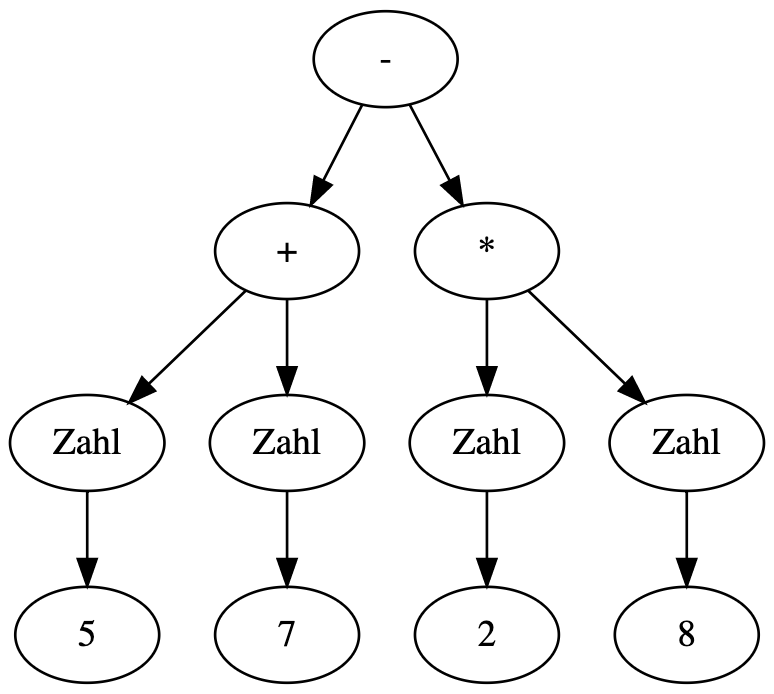
\includegraphics[width=.4\textwidth]{img/syntaxbaum.png}
    \caption{\texttt{5+7-2*8} $\in \AExp$ als verkürzt dargestellter Syntaxbaum}
    \label{fig:syntaxbaum}
\end{figure}

\begin{remark}
    Unterbäume können auch Elemente einer anderen Kategorie sein.
    % B -> (A < A) \in BExp
    % Unterbaum A \in AExp
\end{remark}

\begin{example}
    Division mit Rest
    \begin{itemize}
        \item Eingabe: $a, b > 0$
        \item Ausgabe: $m ,r \geq 0$, $r < b$, $a = m \cdot b + r$
    \end{itemize}
\end{example}

\begin{lstlisting}[language=C, caption=Division mit Rest]
m := 0;
while b <= a do (
    m := m + 1;
    a := a - b
)
r := a
\end{lstlisting}

Die \emph{Semantik} in \texttt{while} wird gegeben durch eine \emph{semantische Funktion}, eine für jede \emph{syntaktische Kategorie}.

Sei $\State = \{ \sigma \mid \sigma: \Var \to \mathbb{Z} \}$, \zb{}
\begin{align*}
    \mathcal{N} : \Num & \to \mathbb{Z} \\
    \mathcal{N}\lsem\texttt{-123}\rsem & = -123
\end{align*}

\begin{align*}
    \A: \underbrace{\AExp}_{\text{``Compiler''}} & \to \underbrace{(\State \to \mathbb{Z})}_{\text{``Interpreter''}} \\
    \A\lsem\texttt{x + x*5}\rsem & = (\sigma \mapsto 6 \cdot \sigma(x)) \quad (\text{da }\texttt{x + x*5} = \texttt{6*x})
\end{align*}

\begin{align*}
    \B : \BExp \to (\State \to \bool) \\
    \B\lsem\texttt{x <= 10}\rsem = \bigg( \sigma \mapsto \begin{cases}
        \true & \sigma(x) \leq 10 \\
        \false & \sigma(x) > 10
    \end{cases} \bigg)
\end{align*}

\[
S: \Stm \to (\State \to \State)
\]

\textbf{Jetzt:} Definition von $\A$ durch Induktion über die Struktur des Syntaxbaums. Die Definition von $\N$ und $\B$ ist eine Übung.

\textbf{Später:} Definition von $S$.



\subsection{Semantik arithmetischer Ausdrücke}

\begin{definition}[Induktive Definition von $\A$]\label{def:Asem}
    Sei $n \in \Num, x \in \Var, \sigma \in \State$ und $a_1, a_2 \in \AExp$. Wir definieren:
    \begin{enumerate}
        \item[(i)] $\A\lsem n \rsem(\sigma) = \N\lsem n \rsem$ \quad\quad (konstante Funktion)
        \item[(ii)] $\A\lsem x \rsem(\sigma) = \sigma(x)$ \quad\quad\quad alternativ: $\A\lsem n \rsem = (\sigma \mapsto \sigma(n))$
        \item[(iii)] $\A\lsem a_1 + a_2 \rsem(\sigma) = \A\lsem a_1 \rsem(\sigma) + \A\lsem a_2 \rsem(\sigma)$ \\[4pt]
        \emph{Bemerkung.} In anderen Sprachen könnte der Aufruf des ersten Summanden Seiteneffekte haben, \dh{} ggf.\ muss man an dieser Stelle aufpassen. In diesem Fall würde der potenziell veränderte Zustand mit zurückgegeben werden.
        \item[(iv)] Analog für Subtraktion
        \item[(v)] Analog für Multiplikation
    \end{enumerate}
\end{definition}

\begin{remark}
    Für die Definition von semantischen Funktionen fordern wir \textbf{Zusammengesetztheit}, \dh{} in der induktiven Definition darf nur auf Bestandteile des Ausdrucks/Syntaxbaums zugegriffen werden.
\end{remark}

\begin{example}
    Führe Negation ein: $\A \to \dots | -A$.

    Erlaubt ist $\A\lsem -a_1 \rsem(\sigma) = 0 - \A\lsem a_1 \rsem(\sigma)$, aber nicht $\A\lsem -a_1 \rsem(\sigma) = \A\lsem 0 - a_1 \rsem(\sigma)$, da der Ausdruck hier um eine Null erweitert wurde.
\end{example}



%%%%%%%%%%%%%%%%%%%%%%%%%%%%%%%%%%%%%%%%%%%%%%%%%%%%%%%%%%%%%%%%%%%%%
\newpage
\hfill 13.05.
%%%%%%%%%%%%%%%%%%%%%%%%%%%%%%%%%%%%%%%%%%%%%%%%%%%%%%%%%%%%%%%%%%%%%

\begin{theorem}
    $\A$ besitzt die folgenden Eigenschaften:
    \begin{enumerate}
        \item Für alle $a \in \AExp$, für alle $\sigma \in \State$ existiert genau eine Zahl $n \in \mathbb{Z}$, sodass $\A\lsem a \rsem (\sigma) = n$. (Voraussetzung: $\sigma$ ist eine totale Funktion.)
        \item $\A$ ist eine totale Funktion.
    \end{enumerate}
\end{theorem}

\begin{proof}[Beweis]
    Skizze:
    \begin{enumerate}
        \item[(b)] folgt aus (a)
        \item[(a)] wird bewiesen durch strukturelle Induktion nach $a$.
    \end{enumerate}
\end{proof}

\par\bigskip
\textbf{Nächste Schritte:}
\begin{enumerate}
    \item[(i)] Der Wert eines Ausdrucks hängt \emph{nur} von den Variablen ab, die in ihm vorkommen. (\secref{section:freeVars})
    \item[(ii)] Was passiert in einem arithmetischen Ausdruck, wenn wir eine Variable durch einen Ausdruck ersetzen ($\leadsto$ \emph{Substitution})? (\secref{section:substitution})
\end{enumerate}



% FREIE VARIABLEN %%%%%%%%%%%%%%%%%%%%%%%%%%%%%%%%%%%%%%%%%%%%%%%%%%%%%%%%%%%%%%%%%%%%%%%%%%%
\subsection{Freie Variablen} \label{section:freeVars}

\begin{definition}[Freie Variablen]
    Sei $a \in \AExp$. $\FV(a)$ (``freie Variablen'') ist die Menge aller Variablen, die in $a$ vorkommen. Formal ist das induktiv definiert:
    \begin{enumerate}
        \item $\FV(n) = \emptyset$ \quad\quad\quad (falls $a = n$ (Zahl))
        \item $\FV(x) = \{ x \}$ \quad\quad (falls $a = x$ (Variable))
        \item $\FV(a_1 \;\square\; a_2) = \FV(a_1) \cup \FV(a_2)$ \quad\quad für $\square \in \{ \texttt{+}, \texttt{-}, \texttt{*} \}$
    \end{enumerate}

    Gebundene Variablen betrachten wir im Kontext der \texttt{while}-Sprache nicht. In anderen Sprachen können aber lokale Variablen \zb{} als solche betrachtet werden.
\end{definition}

\par\medskip
\begin{lemma}
    Sei $a \in \AExp$, sei $\sigma, \sigma' \in \State$, sodass $\sigma(x) = \sigma'(x)$ für alle $x \ in\FV(a)$ gilt.

    Dann gilt:
    \[
    \A\lsem a \rsem(\sigma) = \A\lsem a \rsem(\sigma')
    \]
\end{lemma}

\begin{proof}
    Durch strukturelle Induktion nach $a$.

    \emph{Induktionsanfang:}
    \begin{enumerate}
        \item $a = n$, $n$ Zahl
            \begin{align*}
                \A\lsem a \rsem(\sigma) & = \A\lsem n \rsem(\sigma) \\
                & \overset{\defrefshort{def:Asem}(i)}{=} \N\lsem n \rsem \\
                \\
                \A\lsem a \rsem(\sigma') & = \A\lsem n \rsem(\sigma') \\
                & = \N\lsem n \rsem
            \end{align*}

        \item $a = x$, $x$ Variable
            \begin{align*}
                \A\lsem a \rsem(\sigma) & = \A\lsem x \rsem(\sigma) \\
                & \overset{\defrefshort{def:Asem}(ii)}{=} \sigma(x) \\
                \\
                \A\lsem a \rsem(\sigma') & = \A\lsem x \rsem(\sigma') \\
                & = \sigma'(x) \\
                \\
                \FV(a) & = \FV(x) = \{ x \}
            \end{align*}
            Nach Annahme ist $\sigma(x) = \sigma'(x)$, da $x \in \FV(a)$. Daher folgt
            \[
            \A\lsem a \rsem(\sigma) = \A\lsem a \rsem(\sigma')
            \]
    \end{enumerate}

    \emph{Induktionsschritt:}

    $a = a_1 \;\square\; a_2$ mit $\square \in \{ \texttt{+}, \texttt{-}, \texttt{*} \}$

    \begin{align*}
        \A\lsem a \rsem(\sigma) & = \A\lsem a_1 \;\square\; a_2 \rsem(\sigma) \\
        & = \A\lsem a_1 \rsem(\sigma) \;\square\; \A\lsem a_2 \rsem(\sigma) \\
        \\
        \A\lsem a \rsem(\sigma') & = \A\lsem a_1 \;\square\; a_2 \rsem(\sigma') \\
        & = \A\lsem a_1 \rsem(\sigma') \;\square\; \A\lsem a_2 \rsem(\sigma') \\
        \\
        \FV(a) & = \FV(a_1 \;\square\; a_2) \\
        & = \FV(a_1) \cup \FV(a_2)
    \end{align*}
    Insbesondere gilt, dass $\FV(a_1) \subseteq \FV(a)$ und $\FV(a_2) \subseteq \FV(a)$. Daher folgt:

    Da nach Annahme $\sigma(x) = \sigma(x')$ für alle $x \in \FV(a)$, gilt
    \[
    \sigma(x) = \sigma'(x) \text{ für alle } x \in \FV(a_1)
    \]
    und
    \[
    \sigma(x) = \sigma'(x) \text{ für alle } x \in \FV(a_2)
    \]

    Also gelten nach Induktionsvoraussetzung
    \[
    \A\lsem a_1 \rsem(\sigma) = \A\lsem a_1 \rsem(\sigma') \wedge \A\lsem a_2 \rsem(\sigma) = \A\lsem a_2 \rsem(\sigma')
    \]

    Daher folgt:
    \[
    \A\lsem a_1 \rsem(\sigma) \;\square\; \A\lsem a_2 \rsem(\sigma) = \A\lsem a_1 \rsem(\sigma') \;\square\; \A\lsem a_2 \rsem(\sigma')
    \]
\end{proof}



% SUBSTITUTION %%%%%%%%%%%%%%%%%%%%%%%%%%%%%%%%%%%%%%%%%%%%%%%%%%%%%%%%%%%%%%%%%%%%%%%%%%%%%%%%
\subsection{Substitution}\label{section:substitution}

\begin{definition}[Substitution für Ausdrücke] \label{def:substitutionExp}
    Seien $a, a_0 \in \AExp, \, y \in \Var$. Wir definieren $a[y \mapsto a_0]$ als den arithmetischen Ausdruck, in dem jedes Vorkommen von $y$ in $a$ durch $a_0$ ersetzt wird.

    Formal:
    \begin{enumerate}
        \item[(i)] $n[y \mapsto a_0] = n$
        \item[(ii)] $x[y \mapsto a_0] = \begin{cases} a_0 & \text{falls } x = y \\ x & \text{sonst} \end{cases}$
        \item[(iii)] $(a_1 \;\square\; a_2)[y \mapsto a_0] = a_1[y \mapsto a_0] \;\square\; a_2[y \mapsto a_0]$ \quad\quad für $\square \in \{ +, -, * \}$
    \end{enumerate}
\end{definition}

\begin{example}
    \begin{align*}
        a & = \texttt{x + y*2 - z(x + y)} \\
        \texttt{y} & \mapsto \texttt{4*t + 5} \\
        \\
        a[\texttt{y} \mapsto \texttt{4*t + 5}] & = \texttt{x + (4*t + 5)*2 - z(x + (4*t + 5))}
    \end{align*}
    Es werden die Blätter am Syntaxbaum ersetzt, woraus implizit die Präzedenz klar ist (wodurch die obigen Klammern entstehen).

    Ersetzungen dürfen die zu ersetzende Variable enthalten. Da nur einmal ersetzt wird, ist das in Ordnung.
\end{example}

\begin{definition}[Substitution für Zustände]\label{def:substitutionState}
    Sei $\sigma \in \State, \, x \in \Var, \, n \in \mathbb{Z}$. Dann ist $\sigma[x \mapsto n] \in \State$ der Zustand, der wie folgt definiert ist:
    \begin{align*}
        \sigma[x \mapsto n](z) = \begin{cases}
            n & \text{falls } z = x \\
            \sigma(z) & \text{sonst}
        \end{cases}
    \end{align*}
\end{definition}

\begin{lemma}
    Sei $a, a_0 \in \AExp, \, y \in \Var, \, \sigma \in \State$. Dann gilt:
    \begin{align*}
        \A\lsem a[y \mapsto a_0] \rsem(\sigma) & = \A\lsem a \rsem \Big( \sigma\big[y \mapsto \A\lsem a_0 \rsem(\sigma)\big] \Big)
    \end{align*}
\end{lemma}

Das Lemma setzt Semantik und Syntax in Verbindung: Wir können syntaktisch Variablen durch Teilausdrücke ersetzen und das ist äquivalent dazu, erst den Teilausdruck auszuwerten und mit diesen Wert im Zustand den ursprünglichen Ausdruck auszuwerten.

\begin{example}
    \begin{align*}
    a & = x + y \\
    a_0 & = x * y \\
    \sigma: & \; [x \mapsto 2; y \mapsto 10] \\
    \\
    (x + (x * y))[x \mapsto 2; y \mapsto 10] \quad & \square\; (x + y)[x \mapsto 2; y \mapsto 20] \\
    2 + (2 * 10) \quad & \square\; 2 + 20 \\
    22 \quad & = 22
\end{align*}
\end{example}


\begin{proof}[Beweis]
    Durch strukturelle Induktion nach $a$ (nicht $a_0$!).

    \emph{Induktionsanfang:}
    \begin{enumerate}
        \item $a = n$, $n$ Zahl
            \begin{align*}
                \A\lsem a[y \mapsto a_0] \rsem(\sigma) & = \A\lsem n[y \mapsto a_0] \rsem(\sigma) \\
                & \overset{\defrefshort{def:substitutionExp}(i)}{=} \A\lsem n \rsem(\sigma) \\
                & = n \\
                \\
                \A\lsem n \rsem(\sigma[y \mapsto \A\lsem a_0 \rsem(\sigma)]) & = n \quad\quad \text{(rechte Seite)}
            \end{align*}

        \item $a = x$, $x$ Variable
            \begin{align*}
                \A\lsem x[y \mapsto a_0] \rsem(\sigma) & \overset{\defrefshort{def:substitutionExp}(iii)}{=} \begin{cases}
                    \A\lsem a_0 \rsem(\sigma) & \text{falls } x = y \\
                    \A\lsem x \rsem(\sigma) = \sigma(x) & \text{sonst}
                \end{cases} \\
                \\
                \A\lsem x \rsem(\sigma[y \mapsto \A\lsem a_0 \rsem(\sigma)]) & \overset{\defrefshort{def:substitutionState}}{=} (\sigma[y \mapsto \A\lsem a_0 \rsem(\sigma)])(x) \quad\quad \text{(rechte Seite)} \\
                & = \begin{cases}
                    \A\lsem a_0 \rsem(\sigma) & \text{falls } x = y \\
                    \sigma(x) & \text{sonst}
                \end{cases}
            \end{align*}
    \end{enumerate}

    \emph{Induktionsschritt:} Straight forward.
\end{proof}
%%%%%%%%%%%%%%%%%%%%%%%%%%%%%%%%%%%%%%%%%%%%%%%%%%%%%%%%%%%%%%%%%%%%%
\newpage
\hfill 20.05.
%%%%%%%%%%%%%%%%%%%%%%%%%%%%%%%%%%%%%%%%%%%%%%%%%%%%%%%%%%%%%%%%%%%%%
\subsection{Natürliche operationelle Semantik (``big step'')}
% \subsection{Definition von \texorpdfstring{$\mathcal{S}\lsem \cdot \rsem$}{S[.]}}

$\Asem{\cdot}$ und $\Bsem{\cdot}$ \emph{benutzen} den Zustand $\sigma$ während die Semantik von Anweisungen den Zustand \emph{verändern} soll.

Idee: Definiere $\Ssem{\cdot}$ mithilfe einer Zustandsüberführungerelation.

\begin{definition}
    Sei $s \in \Stm$ eine Anweisungsfolge und seien $\sigma, \sigma' \in \State$ Zustände. Die Zustandsüberführungsrelation
    \[
    \strans{S}{\sigma}{\sigma'}
    \]
    spezifiziert die Beziehung zwischen Startzustand $\sigma$ und dem Endzustand $\sigma'$ gemäß der Anweisungsfolge $S$.
\end{definition}

\begin{remark}[Bedeutung]
    Die Ausführung von $S$ auf Startzustand $\sigma$ terminiert mit Endzustand $\sigma'$.
\end{remark}

\par\medskip
\begin{notation}
    Wir definieren die Zustandsübergangsrelation mithilfe von Schlussregeln. Eine solche Schlussregel besitzt die folgende Form:
    \[
    \frac{\text{Voraussetzung}}{\text{Folgerung}} \leadsto \frac{\strans{S_1}{\sigma_1}{\sigma_1'}, \strans{S_2}{\sigma_2}{\sigma_2'}, \,\dots\, , \strans{S_n}{\sigma_n}{\sigma_n'}}{\strans{S}{\sigma}{\sigma'}}
    \]
    (ggf.\ mit zusätzlichen Bedingungen) wobei $S_1, \dots, S_n$ Bestandteile von $S$ sind.

    Gibt es keine Voraussetzung, nennen wir die Schlussregel ein \emph{Axiom}.
\end{notation}



% SCHLUSSREGELN %%%%%%%%%%%%%%%%%%%%%%%%%%%%%%%%%%%%%%%%%%%%%%%%%%%%%%%%%%%%%%%%%%%%%%%%%%%%%%%
\subsubsection{Schlussregeln für die natürliche Semantik von \texttt{while}}

Im Folgenden schreiben wir $[\cdot]_{\text{ns}}$ um anzuzeigen, dass es sich um die natürliche Semantik handelt.

\begin{enumerate}
    \item Zuweisung $\infruleNs{zuw}$ (Axiom)
    \[
    \frac{}{\strans{x \texttt{ := } a}{\sigma}{\sigma[x \mapsto \Asem{a}(\sigma)]}}
    \]

    \item Skip $\infruleNs{skip}$ (Axiom)
    \[
    \frac{}{\strans{\texttt{skip}}{\sigma}{\sigma}}
    \]

    \item Hintereinanderausführung $\infruleNs{seq}$
    \[
    \frac{\strans{S_1}{\sigma}{\sigma'}, \strans{S_2}{\sigma'}{\sigma''}}{\strans{S_1 \texttt{;} S_2}{\sigma}{\sigma''}}
    \]
    Dabei können $S_1$ und $S_2$ zusammengesetzte Anweisungen sein.

    \item Verzweigung $\infruleNs[\true]{if}$
    \[
    \frac{\strans{S_1}{\sigma}{\sigma'}}{\strans{\texttt{if } b \texttt{ then } S_1 \texttt{ else } S_2}{\sigma}{\sigma'}}
    \]
    falls $\Bsem{b}(\sigma) = \true$. Dabei muss $S_2$ nicht terminieren.

    \item Verzweigung $\infruleNs[\false]{if}$
    \[
    \frac{\langle S_2, \sigma \rangle \to \sigma'}{\langle \texttt{if } b \texttt{ then } S_1 \texttt{ else } S_2, \sigma \rangle \to \sigma'}
    \]
    falls $\Bsem{b}(\sigma) = \false$. Dabei muss $S_1$ nicht terminieren.

    \item Schleife $\infruleNs[\true]{while}$
    \[
    \frac{\langle S, \sigma \rangle \to \sigma', \langle \texttt{while } b \texttt{ do } S, \sigma' \rangle \to \sigma''}{\langle \texttt{while } b \texttt{ do } S, \sigma \rangle \to \sigma''}
    \]
    falls $\Bsem{b}(\sigma) = \true$. Im Allgemeinen kann es sein, dass die Schleife nicht terminiert. Deshalb müssen wir diesen Fall in der Definition der semantischen Funktion beachten. Das bedeutet, diese Relation ist nicht total.

    \item Schleife $\infruleNs[\false]{while}$
    \[
    \frac{\text{ }}{\langle \texttt{while } b \texttt{ do } S, \sigma \rangle \to \sigma}
    \]
    falls $\Bsem{b}(\sigma) = \false$.
\end{enumerate}

\par\bigskip
\par\bigskip
Wie ist die Zustandsüberführungsfunktion überhaupt definiert?

\begin{definition}
    Sei $S \in \Stm$ ein Programm und seien $\sigma, \sigma' \in \State$. Dann gilt
    \[
    \langle S, \sigma \rangle \to \sigma'
    \]
    gdw.\ ein \emph{endlicher Ableitungsbaum} dafür existiert.

    Der Ableitungsbaum entsteht durch wiederholte Anwendung der Schlussregeln. Die Wurzel ist $\langle S, \sigma \rangle \to \sigma'$, die Blätter sind Axiome, die Knoten entsprechen der korrekten Anwendung der Schlussregeln.
\end{definition}

\begin{example}
    Sei $\sigma \in \State$ mit $\sigma(x) = 1$ und $\sigma(y) = 5$.

    Behauptung: $\langle (z := x; x := y); y := z, \sigma \rangle \to \sigma[z \mapsto 1][x \mapsto 5][y \mapsto 1]$

    Nun müssen wir den endlichen Ableitungsbaum erzeugen.


    \begin{enumerate}
        \item $\infruleNs{seq}$
            \[
            \frac{\langle z := x; x := y, \sigma \rangle \to \sigma', \langle y := z, \sigma' \rangle \to \sigma[z \mapsto 1][x \mapsto 5][y \mapsto 1]}{\langle \underbrace{(z := x; x := y)}_{s_1}; \underbrace{y := z}_{S_2}, \sigma \rangle \to \sigma[z \mapsto 1][x \mapsto 5][y \mapsto 1]}
            \]

            Welches $\sigma'$ brauchen wir? $\leadsto \sigma[z \mapsto 1][x \mapsto 5]$. Somit erhalten wir
            \[
            \frac{\langle z := x; x := y, \sigma \rangle \to \sigma[z \mapsto 1][x \mapsto 5], \langle y := z, \sigma[z \mapsto 1][x \mapsto 5] \rangle \to \sigma[z \mapsto 1][x \mapsto 5][y \mapsto 1]}{\langle \underbrace{(z := x; x := y)}_{S_1}; \underbrace{y := z}_{S_2}, \sigma \rangle \to \sigma[z \mapsto 1][x \mapsto 5][y \mapsto 1]}
            \]

        \item $\infruleNs{zuw}$ für den rechten Teil
            \[
            \frac{\Asem{z}(\sigma[z \mapsto 1][x \mapsto 5]) \overset{?}{=} 1}{\langle y := z, \sigma[z \mapsto 1][x \mapsto 5] \rangle \to \sigma[z \mapsto 1][x \mapsto 5][y \mapsto 1]}
            \]

            \[
            \Asem{z}(\sigma[z \mapsto 1][x \mapsto 5]) \overset{Def}{=} \sigma[z \mapsto 1][x \mapsto 5](z) \overset{Def}{=} 1
            \]

        \item $\infruleNs{seq}$
            \[
            \frac{\langle z := x, \sigma \rangle \to \sigma[z \mapsto 1], \langle x := y, \sigma[z \mapsto 1] \rangle \to \sigma[z \mapsto 1][x \mapsto 5]}{\langle z := x; x := y, \sigma \rangle \to \sigma[z \mapsto 1][x \mapsto 5]}
            \]

            Ab hier analog zum rechten Teil (mit zwei Mal $\infruleNs{zuw}$).
    \end{enumerate}
\end{example}

\par\bigskip
\begin{remark}[Rechtseindeutigkeit / Determiniertheit]
    Es ist noch nicht klar, dass ``$\to$'' \emph{rechtseindeutig} ist. D.\,h. möglicherweise existiert ein Programm $S$, ein Startzustand $\sigma$ und Zustände $\sigma_1 \neq \sigma_2 \in \State$, sodass sowohl
    \[
    \langle S, \sigma \rangle \to \sigma_1 \text{ als auch } \langle S, \sigma \rangle \to \sigma_2
    \]
    gilt. Daher muss die Rechtseindeutigkeit bzw. \emph{Determiniertheit} bewiesen werden!
\end{remark}

\par\medskip
\begin{remark}[Ableitungsbaum]
    Der Ableitungsbaum ist statisch. D.\,h. man kann nicht erkennen, in welcher Reihenfolge die Schlussregeln angewendet werden.
\end{remark}



%%%%%%%%%%%%%%%%%%%%%%%%%%%%%%%%%%%%%%%%%%%%%%%%%%%%%%%%%%%%%%%%%%%%%
\newpage
\hfill 27.05.
%%%%%%%%%%%%%%%%%%%%%%%%%%%%%%%%%%%%%%%%%%%%%%%%%%%%%%%%%%%%%%%%%%%%%
\begin{definition}
    Sei $S$ ein Programm und $\sigma$ ein Startzustand. Das Programm $S$ \emph{terminiert} bei Startzustand $\sigma$ falls ein $\sigma'$ existiert, sodass $\strans{S}{\sigma}{\sigma'}$ gilt.

    ? Analog \emph{terminiert $S$ nicht} bei Startzustand $\sigma$.

    Das Programm $S$ \emph{terminiert immer}, falls $S$ für jeden Startzustand $\sigma$ terminiert. $S$ \emph{terminiert nie}, falls $S$ für keinen Startzustand $\sigma$ terminiert.
\end{definition}

\begin{definition}
    Seien $S_1, S_2$ zwei Programme. $S_1$ und $S_2$ heißen \emph{semantisch äquivalent}, falls für alle Zustände $\sigma, \sigma'$ gilt
    \[
    \strans{S_1}{\sigma}{\sigma'} \Leftrightarrow \strans{S_2}{\sigma}{\sigma'}
    \]
\end{definition}

\begin{example}
    Die Programme
    \[
    S_1 = \texttt{while b do S}
    \]
    und
    \[
    S_2 = \texttt{if b then (S; while b do S) else skip}
    \]
    sind semantisch äquivalent.
\end{example}
\begin{proof}
    Seien $\sigma, \sigma'$ Zustände. Z.\,z.: $\strans{S_1}{\sigma}{\sigma'} \Leftrightarrow \strans{S_2}{\sigma}{\sigma'}$.

    \begin{enumerate}
        \item ``$\Rightarrow$''

            Angenommen, es gilt $\strans{S_1}{\sigma}{\sigma'}$. Also existiert nach Definition ein endlicher Ableitungsbaum für $\strans{S_1}{\sigma}{\sigma'}$.
            \begin{enumerate}
                \item $\Bsem{b}(\sigma) = \true$

                    Dann hat der Ableitungsbaum $T_1$ die Form
                    \begin{align*}
                        \infruleNs[\true]{while}\;
                        \cfrac{
                            \cfrac{T_a}{\strans{S}{\sigma}{\sigma''}}
                            \;,\;
                            \cfrac{T_b}{\strans{\texttt{while b do S}}{\sigma''}{\sigma'}}
                        }{
                            \strans{\texttt{while b do S}}{\sigma}{\sigma'}
                        }
                    \end{align*}

                    Z.\,z.:\ es existiert ein endlicher Ableitungsbaum für $\strans{S_2}{\sigma}{\sigma'}$
                    \begin{align*}
                        \infruleNs[\true]{if}\;
                        \cfrac{
                            \infruleNs{seq}\;
                            \cfrac{
                                \cfrac{T_a}{\strans{S}{\sigma}{\sigma''}}
                                ,
                                \cfrac{T_b}{\strans{\texttt{while b do S}}{\sigma''}{\sigma'}}
                            }{
                                \strans{\texttt{S; while b do S}}{\sigma}{\sigma'}
                            }
                        }{
                            \strans{\texttt{if b then (S; while b do S) else skip}}{\sigma}{\sigma'}
                        }
                        \quad
                        \Bsem{b}(\sigma) = \true
                    \end{align*}

                \item $\Bsem{b}(\sigma) = \false$

                    Dann hat $T_1$ die Form
                    \begin{align*}
                        \infruleNs[\false]{while}\;
                        \cfrac{}{
                            \strans{\texttt{while b do S}}{\sigma}{\sigma}
                        }
                        \quad
                        \Bsem{b}(\sigma) = \false
                    \end{align*}
                    Dieses Axiom ist wahr, gdw. $\sigma = \sigma'$.

                    Z.\,z.: Es existiert ein Ableitungsbaum für $\strans{S_2}{\sigma}{\sigma}$.
                    \begin{align*}
                        \infruleNs[\false]{if}\;
                        \cfrac{
                            \infruleNs{skip}\;
                            \cfrac{}{\strans{\texttt{skip}}{\sigma}{\sigma}}
                        }{
                            \strans{\texttt{if b then (S; while b do S) else skip}}{\sigma}{\sigma}
                        }
                        \quad
                        \Bsem{b}(\sigma) = \false
                    \end{align*}
            \end{enumerate}

        \item ``$\Leftarrow$''

            Analog.
    \end{enumerate}
\end{proof}

\begin{lemma}
    Die natürliche Semantik der \texttt{while}-Sprache ist \emph{determiniert}, \dh{} für alle Anweisungen $S$ und Zustände $\sigma, \sigma_1, \sigma_2$ gilt:

    Wenn $\strans{S}{\sigma}{\sigma_1}$ und $\strans{S}{\sigma}{\sigma_2}$, dann $\sigma_1 = \sigma_2$.
\end{lemma}
\begin{proof}
    Durch strukturelle Induktion nach Tiefe des Ableitungsbaums. (Übung)
\end{proof}


\begin{definition}
    Die semantische Funktion $\mathcal{S}_{\text{ns}}: \State \to (\State \to \State)$ ist definiert als
    \begin{align*}
        \mathcal{S}_{\text{ns}}\lsem S \rsem(\sigma) = \begin{cases}
            \sigma' & \text{falls } \exists\; \sigma': \strans{S}{\sigma}{\sigma'} \\
            \bot & \text{sonst}
        \end{cases}
    \end{align*}
\end{definition}
\subsection{Strukturelle operationelle Semantik (``small step'')}

Hier geht es um die genaue Reihenfolge der Schritte bei der Ausführung. Das ist bespielsweise nützlich bei der parallelen Ausführungen eines Programms.

Wir definieren wieder eine Zustandsüberführungsrelation ``$\Rightarrow$''. Sie hat die Form
\begin{align*}
    \langle S, \sigma \rangle & \Rightarrow \langle S', \sigma' \rangle \tag{*} \\
    \text{oder} \\
    \langle S, \sigma \rangle & \Rightarrow \sigma' \tag{**}
\end{align*}

Interpretation:
\begin{enumerate}
    \item[(*)] Ausführung ist noch nicht vorbei, sondern erreicht in \emph{einem Schritt} die \emph{Zwischenkonfiguration} $\langle s', \sigma' \rangle$.
    \item[(**)] Ausführung ist nach einem Schritt vorbei und erreicht den Endzustand $\sigma'$.
\end{enumerate}



Wir definieren $\Rightarrow$ durch folgende Schlussregeln. Im Folgenden schreiben wir $[\cdot]_{\text{sos}}$ um anzuzeigen, dass es sich um die strukturelle operationelle Semantik handelt.


\begin{enumerate}
    \item $\infruleSos{zuw}$
    \[
    \langle x \texttt{ := } a, \sigma \rangle \Rightarrow \sigma[x \mapsto \Asem{a}(\sigma)]
    \]

    \item $\infruleSos{skip}$
    \[
    \langle \texttt{skip}, \sigma \rangle \Rightarrow \sigma
    \]

    \item $\infruleSos[1]{seq}$
    \begin{align*}
        \frac{
            \langle S_1, \sigma \rangle \Rightarrow \langle S_1', \sigma' \rangle
        }{
            \langle S_1\texttt{;} S_2, \sigma \rangle \Rightarrow \langle S_1'\texttt{;} S_2, \sigma' \rangle
        }
    \end{align*}

    \item $\infruleSos[2]{seq}$
    \begin{align*}
        \frac{
            \langle S_1, \sigma \rangle \Rightarrow \sigma'
        }{
            \langle S_1\texttt{;} S_2, \sigma \rangle \Rightarrow \langle S_2, \sigma' \rangle
        }
    \end{align*}


    \item $\infruleSos[\true]{if}$
    \begin{align*}
        \langle \texttt{if } b \texttt{ then } S_1 \texttt{ else } S_2, \sigma \rangle \Rightarrow \langle S_1, \sigma \rangle
    \end{align*}
    falls $\Bsem{b}(\sigma) = \true$

    \item $\infruleSos[\false]{if}$
    \begin{align*}
        \langle \texttt{if } b \texttt{ then } S_1 \texttt{ else } S_2, \sigma \rangle \Rightarrow \langle S_2, \sigma \rangle
    \end{align*}
    falls $\Bsem{b}(\sigma) = \false$

    \item $\infruleSos{while}$
    \[
    \langle \texttt{while } b \texttt{ do } S, \sigma \rangle \Rightarrow \langle \texttt{if } b \texttt{ then } \texttt{(S; while } b \texttt{ do } S) \texttt{ else skip}, \sigma \rangle
    \]
\end{enumerate}

\begin{definition}
    Sei $S$ eine Anweisung und $\sigma$ ein Zustand.

    Eine Ableitungsfolge für $\langle S, \sigma \rangle$ ist entweder
    \begin{enumerate}
        \item eine endliche Folge $\gamma_0 \Rightarrow \gamma_1 \Rightarrow \dots \Rightarrow \gamma_k$ von Konfigurationen, sodass $\gamma_0 = \langle S, \sigma \rangle$ ist, $\gamma_i \Rightarrow \gamma_{i+1}$ für $0, \dots, k-1$ gilt und $\gamma_k$ entweder ein Zustand $\sigma'$ oder eine Konfiguration $\langle S', \sigma' \rangle$ ist, für die es mit $\Rightarrow$ nicht weiter geht \emph{(steckengebliebene Konfiguration)}.

        \item eine unendliche Folge $\gamma_0 \Rightarrow \gamma_1 \Rightarrow \dots$ von Konfigurationen mit $\gamma_0 = \langle S, \sigma \rangle$ mit $\gamma_i \Rightarrow \gamma_{i+1}$ für $i \geq 0$.
    \end{enumerate}
\end{definition}

\par\medskip
\begin{notation}
    Wir schreiben

    $\gamma_0 \Rightarrow^i \gamma'$ für ``$\gamma'$ geht aus $i$ Schritten hervor'' und

    $\gamma_0 \Rightarrow^* \gamma'$ für ``$\gamma'$ geht aus endlich vielen Schritten hervor'' (auch null).
\end{notation}



%%%%%%%%%%%%%%%%%%%%%%%%%%%%%%%%%%%%%%%%%%%%%%%%%%%%%%%%%%%%%%%%%%%%%
\newpage
\hfill 03.06.
%%%%%%%%%%%%%%%%%%%%%%%%%%%%%%%%%%%%%%%%%%%%%%%%%%%%%%%%%%%%%%%%%%%%%

\begin{example}
    Sei $\sigma$ ein Zustand mit $\sigma(x) = 5, \sigma(y) = 7$. Betrachte die Auswertung von \texttt{(z := x; x := y); y = z;} in der SOS für Startzustand $\sigma$.

    \begin{align*}
        & \langle \texttt{(z := x; x := y); y = z;}, \sigma \rangle \\
        \overset{\infruleSos[1]{seq}}{\Rightarrow} \quad & \langle \texttt{x := y; y := z}, \sigma[z \mapsto 5] \rangle \tag{i} \\
        \overset{\infruleSos[2]{seq}}{\Rightarrow} \quad & \langle \texttt{y := z}, \sigma[z \mapsto 5][y \mapsto 7] \rangle \tag{ii} \\
        \overset{\infruleSos{zuw}}{\Rightarrow} \quad & \sigma[z \mapsto 5][x \mapsto 7][y \mapsto 5]
    \end{align*}

    zu (i):
    \begin{align*}
        \infruleSos[1]{seq}\; \cfrac{
            \infruleSos[2]{seq}\; \cfrac{
                \infruleSos{zuw}\; \cfrac{}{
                    \stranssos{\texttt{z := x}}{\sigma}{\sigma[z \mapsto 5]}
                }
            }{
                \stranssos{\texttt{z := x; x := y}}{\sigma}{\langle \texttt{x := y}, \sigma[z \mapsto 5] \rangle}
            }
        }{
            \stranssos{\texttt{(z := x; x := y); y := z}}{\sigma}{\langle \texttt{x := y; y := z}, \sigma[z \mapsto 5] \rangle}
        }
    \end{align*}

    zu (ii):
    \begin{align*}
        \infruleSos[2]{seq}\; \cfrac{
            \infruleSos{zuw}\; \cfrac{}{
                \stranssos{x :=y}{\sigma[z \mapsto 5]}{\langle y :=z, \sigma[z \mapsto5][x \mapsto 7] \rangle}
            }
        }{
            \stranssos{x :=y; y :=z}{\sigma[z \mapsto 5]}{\langle y :=z, \sigma[z \mapsto5][x \mapsto 7] \rangle}
        }
    \end{align*}
\end{example}



\subsection{Eigenschaften der SOS}

\begin{lemma}
    Seiten $S_1, S_2$ Anweisungen, $\sigma, \sigma''$ Zustände und $k \in \mathbb{N}$.
    Dann gilt: Falls $\langle S_1; S_2, \sigma \rangle \Rightarrow^k \sigma''$ gilt, es existieren zwei Zahlen $k_1, k_2 \in \mathbb{N}$ mit
    \[
        \langle S_1, \sigma \rangle \Rightarrow^{k_1} \sigma'
        \;,\quad
        \langle S_2, \sigma' \rangle \Rightarrow^{k_2} \sigma''
    \]
    und
    \[
        k_1 + k_2 = k
    \]
\end{lemma}
\begin{proof}
    Induktion nach $k$.

    \emph{Induktionsanfang:}
    \begin{enumerate}
        \item $k = 1$: Voraussetzung kann dafür nicht erfüllt sein, also stimmt die Aussage.
        \item $k = 2$: Wie kann $\langle S_1; S_2, \sigma \rangle \Rightarrow^2 \sigma''$ gelten?
            Das kann nur sein, wenn im ersten Schritt $\infruleSos[2]{seq}$ augewendet wird. D.\,h. die Schlussregel
            \[
                \frac{\stranssos{S_1}{\sigma}{\sigma'}}{\stranssos{S_1; S_2}{\sigma}{\langle S_2, \sigma' \rangle}}
            \]
            wurde erfüllt für ein $\sigma'$.

            Wir wissen also, es existiert ein Zwischenzustand $\sigma'$ mit $\stranssos{S_1}{\sigma}{\sigma'}$ und erster Schritt von $\langle S_1; S_2, \sigma \rangle \Rightarrow^2 \sigma''$ ist $\langle S_1; S_2, \sigma \rangle \Rightarrow \langle S_2, \sigma' \rangle$
            Der zweite Schritt $\langle S_1; S_2, \sigma \rangle \Rightarrow^2 \sigma''$ muss jetzt aber der Form $\langle S_2, \sigma' \rangle \Rightarrow \sigma''$ sein.

            D.\,h. die Aussage gilt mit $k_1 = 1, k_2 = 1$ und $\sigma'$.
    \end{enumerate}

        \par\bigskip
    \emph{Induktionsschritt:} $k - 1 \mapsto k$ mit $k \geq 3$

    Betrachten den ersten Schritt $\langle S_1; S_2, \sigma \rangle \Rightarrow^k \sigma''$.
    Zwei Fälle
    \begin{enumerate}
        \item $\infruleSos[1]{seq}$ Der erste Schritt hat die Form $\langle S_1; S_2, \sigma \rangle \Rightarrow^k \langle S_1'; S_2, \sigma''' \rangle$

            Dann muss aber gelten $\langle S_1'; S_2, \sigma''' \rangle \Rightarrow^{k-1} \sigma''$.
            Nach IV existiert $k_1', k_2' \in \mathbb{N}, \sigma'$, sodass $\langle S_1',  \sigma''' \rangle \Rightarrow^{k_1'} \sigma'$ und $\langle S_2',  \sigma' \rangle \Rightarrow^{k_2'} \sigma''$ und $k_1' + k_2' = k - 1$.

            Da wir im ersten Schritt $\infruleSos[1]{seq}$ angewandt haben, muss die Schlussregel dafür erfüllt gewesen sein, \dh{} es gilt $\langle S_1, \sigma \rangle \Rightarrow \langle S_1', \sigma''' \rangle$. Also gilt auch $\langle S_1', \sigma \rangle \Rightarrow^{k_1'} \sigma'$ also $\langle S_1, \sigma \rangle \Rightarrow^{k_1+1} \sigma'$.

            Also gilt die Aussage für $k_1 + 1, k_2 = k_2', \sigma'$.
        \item $\infruleSos[2]{seq}$ Der erste Schritt hat die Form $\langle S_1; S_2, \sigma \rangle \Rightarrow \langle S_2, \sigma' \rangle$ und es gilt $\langle S_1, \sigma \rangle \Rightarrow \sigma'$.

            Also gilt die Aussage für $k_1 = 1, k_2 = k - 1, \sigma'$.
    \end{enumerate}
\end{proof}


\begin{lemma}[Determinierheit]
    SOS ist \emph{determiniert}. Anders als bei der natürlichen Semantik müssen auch alle Zwischenzustände gleich sein, \dh{}

        Für jedes $S, \sigma$ existiert gibt es eine Ableitungsfolge, die mit $\langle S, \sigma \rangle$ beginnt.
\end{lemma}


\begin{definition}[Semantische Äquivalenz]
    Seien $S_1, S_2$ zwei Anweisungen. $S_1, S_2$ heißen \emph{semantische äquivalent} gdw. folgendes für allen Zustände $\sigma$ gilt:

    \begin{enumerate}
        \item Für alle steckengebliebenen Konfigurationen $\gamma$ und alle Endzustände $\sigma'$ gilt
            \[
                \langle S_1, \sigma \rangle \Rightarrow^* \gamma \Leftrightarrow \langle S_2, \sigma \rangle \Rightarrow^* \gamma
            \]
            und
            \[
                \langle S_1, \sigma \rangle \Rightarrow^* \sigma' \Leftrightarrow \langle S_2, \sigma \rangle \Rightarrow^* \sigma'
            \]
        \item Es existiert eine undendliche Ableitungsfolge für $\langle S_1, \sigma \rangle$ gdw. es existiert eine unendliche Folge für $\langle S_2, \sigma \rangle$.
    \end{enumerate}
\end{definition}

\par\medskip
\begin{example}
    \texttt{$S_1$; ($S_2$; $S_3$)} und \texttt{($S_1$; $S_2$); $S_3$} sind semantische äquivalent.
\end{example}



\subsection{Semantische Funktion $\mathcal{S_{\text{sos}}}$}

\begin{definition}
    Definiere $\mathcal{S_{\text{sos}}}: \Stm \to (\State \to \State)$ als
    \[
        \mathcal{S_{\text{sos}}}\lsem S \rsem(\sigma) = \begin{cases}
            \sigma' & \text{falls} \langle S, \sigma \rangle \Rightarrow^* \sigma' \\
            \bot & \text{sonst}
        \end{cases}
    \]

    Diese Funktion ist wohldefiniert, da SOS determiniert ist.
\end{definition}

\begin{theorem}
    Sei $S$ eine Anweisung und seien $\sigma, \sigma'$ Zustände. Dann gilt
    \[
        \mathcal{S_{\text{ns}}}\lsem S \rsem(\sigma) = \sigma'
        \quad\Leftrightarrow\quad
        \mathcal{S_{\text{sos}}}\lsem S \rsem(\sigma) = \sigma'
    \]

    D.\,h. SOS und NS sind äquivalent für unser \emph{konkretes Beispiel} der \texttt{while}-Sprache.
\end{theorem}

\begin{proof}
    Zwei Richtungen:
    \begin{enumerate}
        \item ``$\Rightarrow$'': $\mathcal{S_{\text{ns}}}\lsem S \rsem(\sigma) = \sigma' \Rightarrow \mathcal{S_{\text{sos}}}\lsem S \rsem(\sigma) = \sigma'$

            \dh{} $\langle S, \sigma \rangle \to \sigma' \implies \langle S, \sigma \rangle \Rightarrow^* \sigma'$

            Wir wissen $\langle S, \sigma \rangle \to \sigma'$, \dh{} es existiert ein endliche Ableitungsbaum $T$ dafür. Mache Induktion nach der Tiefe von $T$.

            \par\medskip
            \emph{Induktionsanfang:} $T$ hat Tiefe 0, \dh{} $T$ besteht nur aus einer Wurzel. Das bedeutet, $\langle S, \sigma \rangle \to \sigma'$ erfolgt durch Anwendung eines Axioms. Davon gibt es drei Stück: $\infruleNs{zuw}, \infruleNs{skip}, \infruleNs[\false]{while}$

            Exemplarisch für $\infruleNs[\false]{while}$:

            Wir wissen $S$ hat die Form \texttt{while $b$ do $S$} und $\Bsem{b}(\sigma) = \false$. D.\,h. $T$ hat die Form
            \[
                \frac{}{
                    \strans{\texttt{while $b$ do $S'$}}{\sigma}{\underbrace{\sigma'}_{\sigma}}
                }
            \]
            Jetzt gilt
            \begin{align*}
                & \langle \texttt{while $b$ do $S'$}, \sigma \rangle \\
                \overset{\infruleSos{while}}{\Rightarrow} \quad & \langle \texttt{if $b$ then ($S'$; while $b$ do $S'$) else skip} , \sigma \rangle \\
                \overset{\infruleSos[\false]{if}}{\Rightarrow} \quad & \langle \texttt{skip}, \sigma \rangle \quad\quad \text{da } \Bsem{b}(\sigma) = \false \\
                \overset{\infruleSos{skip}}{\Rightarrow} \quad & \sigma \\
            \end{align*}
            Also $\langle \texttt{while $b$ do $S'$}, \sigma \rangle \Rightarrow^* \sigma$ wie gewünscht.

%%%%%%%%%%%%%%%%%%%%%%%%%%%%%%%%%%%%%%%%%%%%%%%%%%%%%%%%%%%%%%%%%%%%%
\newpage
\hfill 10.06.
%%%%%%%%%%%%%%%%%%%%%%%%%%%%%%%%%%%%%%%%%%%%%%%%%%%%%%%%%%%%%%%%%%%%%

            \par\bigskip
            \emph{Induktionsschritt:}
            \begin{enumerate}
                \item $\infruleNs[\true]{while}$
                \item $\infruleNs[*]{if}$
                \item $\infruleNs{seq}$
            \end{enumerate}

            Wir machen exemplarisch (a).

            Es gilt $\strans{S}{\sigma}{\sigma'}$, \dh{} $T$: \[
                \frac{
                    \cfrac{T_1}{\strans{S'}{\sigma}{\sigma''}}
                    \;,\quad
                    \cfrac{T_2}{\strans{\texttt{while b do S'}}{\sigma''}{\sigma'}}
                }{
                    \strans{\texttt{while b do S'}}{\sigma}{\sigma'}
                }
            \]
            $T_1$ und $T_2$ existieren, da $T$ existiert. Außerdem sind die Höhen von $T_1, T_2 < $ Höhe von $T$. Also folgt aus der IV, dass

            wegen $\strans{S'}{\sigma}{\sigma''}$ auch \[
                \langle S', \sigma \rangle \Rightarrow^* \sigma''
            \]
            und wegen $\strans{S'}{\sigma''}{\sigma'}$ auch \[
                \langle S, \sigma'' \rangle \Rightarrow^* \sigma'
            \]
            gilt.

            \begin{align*}
                \langle \texttt{while b do S}, \sigma \rangle \Rightarrow & \quad \langle \texttt{if b then (S'; while b do S') else skip}, \sigma \rangle \\
                \overset{\infruleSos[\true]{if}}{\Rightarrow} & \quad \langle \texttt{S'; while b do S'}, \sigma \rangle \quad \text{weil } \Bsem{b}(\sigma) = \true \\
                \overset{\text{IV}}{\Rightarrow^*} & \quad \sigma' \quad \text{(Übung)}
            \end{align*}

        \item ``$\Leftarrow$'': Übung
    \end{enumerate}
\end{proof}



\subsection{Erweiterungen der \texttt{while}-Sprache}


\subsubsection{Programmabbruch}

Füge eine neue Anweisung \texttt{abort} zur Sprache hinzu. Die Bedeutung ist, dass das Programm fehlerhaft abgebrochen wird.
\[
    S \to \dots \;\vert\; \texttt{abort}
\]
Wir fügen für \texttt{abort} \emph{keine neuen Schlussregeln} hinzu -- weder für die NS noch die SOS).

\begin{example}
    Wir betrachten folgende Anweisung, in der die Schleife die Fakultät berechnet:

    $S =$ \texttt{if $\neg(x \geq 1)$ then abort else (y := 1; while $\neg(x = 1)$ do (y := y * x; x := x - 1))}

    \par\bigskip
    \hrule
    \emph{Wie sieht es bei der NS aus?}

    Sie $\sigma(x) = -1$. Wie sieht dann der Ableitungsbaum aus?
    \begin{align*}
        \infruleNs[\true]{if}\; \frac{
            \cfrac{
                T
            }{
                \strans{\texttt{abort}}{\sigma}{\sigma'}
            }
        }{
            \strans{S}{\sigma}{\sigma'}
        }
    \end{align*}
    Dabei existiert $T$ nicht! Daraus folgt \[
        \Ssem{S}(\sigma) = \bot
    \] (für unseren konkreten Zustand $\sigma$).

    $S$ ist \textbf{semantisch äquivalent} zu

    $S' =$ \texttt{if $\neg(x \geq 1)$ then (while true do skip) else (y := 1; while $\neg(x = 1)$ do (y := y * x; x := x - 1))}

    denn auch für \texttt{while true do skip} existiert auch kein endlicher Ableitungsbaum. D.\,h. in der natürlichen Semantik können wir nicht zwischen Abbruch und Endlossschleife unterscheiden.

    \par\bigskip
    \hrule
    \emph{Wie sieht es bei der SOS aus?}
    \begin{align*}
        \langle S, \sigma \rangle \overset{\infruleSos[\true]{if}}{\Rightarrow} \langle \texttt{abort}, \sigma \rangle
    \end{align*}
    Die rechte Konfiguration ist eine steckengebliebene Konfiguration.
    \begin{align*}
        \langle S', \sigma \rangle \overset{\infruleSos[\true]{if}}{\Rightarrow} & \quad \langle \texttt{while true do skip}, \sigma \rangle \\
        \Rightarrow^* & \quad \langle \texttt{while true do skip}, \sigma \rangle \\
        \Rightarrow^* & \quad \dots
    \end{align*}
    D.\,h. in der SOS sind $S$ und $S'$ \textbf{nicht semantisch äquivalent}.
\end{example}



\subsubsection{Blöcke und lokale Variablen}

\emph{Idee:} Erlaube Definition lokaler Variablen innerhalb eines Bereichs.

\begin{align*}
    S & \to \dots \;\vert\; \texttt{begin $D_V$ $S$ end} \\
    D_V & \to \texttt{var} \text{ Var } \texttt{:= A; $D_V$} \;\vert\; \varepsilon
\end{align*}

$D_V$ entspricht der syntaktischen Kategorie Dec$_V$.

\begin{example}
Betrachte
\begin{lstlisting}[language=Pascal]
begin
    var y := 1;
    x := 1;
    begin
        var x := 2;
        y := x + 1  (* (1) 2 + 1 *)
    end
    y := y + x (* (2) 3 + 1 *)
end
\end{lstlisting}

In (1) und (2) überdeckt das lokale $x$ das globale $x$ \emph{in diesem Block}.
\end{example}



\subsubsection{Formalisierung lokaler Blöcke in der NS}

\begin{definition}
    Sei $D_V$ eine Variablendeklaration. Die Menge der in ihr deklarierten Variablen $\DV(D_V)$ ist definiert als:
    \begin{align*}
        \DV(\varepsilon) & := \varnothing \\
        \DV(\texttt{var } x := a \texttt{; } D_V') & := \{ x \} \cup \DV(D_V')
    \end{align*}

    Wir führen eine neue Relation ``$\to_D$'' ein. Sie hat die Form \[
        \langle D_V, \sigma \rangle \to_D \sigma'
    \]
    wobei $\sigma'$ ein lokaler Zustand ist.
\end{definition}



\subsubsection{Schlussregeln für $D_V$, $\to_D$ und Blöcke}

\begin{align*}
    \langle \varepsilon, \sigma \rangle \to_D \sigma \\
    \\
    \frac{
        \langle D_V, \sigma[x \mapsto \Asem{a}(\sigma)] \rangle \to_D \sigma'
    }{
        \langle \texttt{var } x := a \texttt{; } D_V, \sigma \rangle \to_D \sigma'
    } \\
    \\
    \frac{
        \langle D_V, \sigma \rangle \to_D \sigma'', \langle S, \sigma'' \rangle \to \sigma'
    }{
        \langle \texttt{begin $D_V$ $S$ end}, \sigma \rangle \to \sigma'[\DV(D_V) \mapsto \sigma]
    }
\end{align*}
wobei
\begin{align*}
    \sigma'[X \mapsto \sigma](x) = \begin{cases}
        \sigma(x) & \text{falls } x \in X \\
        \sigma'(x) & \text{falls } x \not\in X
    \end{cases}
\end{align*}
\dh{} alle lokale deklarierten Variablen werden auf ihren ursprünglichen Wert zurückgesetzt.


%%%%%%%%%%%%%%%%%%%%%%%%%%%%%%%%%%%%%%%%%%%%%%%%%%%%%%%%%%%%%%%%%%%%%
\newpage
\hfill 17.06.
%%%%%%%%%%%%%%%%%%%%%%%%%%%%%%%%%%%%%%%%%%%%%%%%%%%%%%%%%%%%%%%%%%%%%

\subsubsection{Unterprogramme / Prozeduren / Subroutine / Methode}

Wir wollen ein neues Sprachkonstrukt für \texttt{while} einführen: Prozeduren (wie in Pascal).

Dazu erweitern wir im ersten Schritt die Grammatik:
\begin{align*}
    S & \to \dots \;\vert\; \texttt{begin $D_V$ $D_p$ $S$ end} \;\vert\; \texttt{call $p$} \\
    D_p & \to \texttt{proc $p$ is $S$; $D_p$} \;\vert\; \varepsilon
\end{align*}

$p$ steht für den Bezeichner der Prozedur. $D_p$ entspricht der syntaktischen Kategorie $p_{\text{Name}}$.
$D_p$ entspricht der syntaktischen Kategorie für Unterprogramm-Deklarationen.

\par\medskip
\begin{example}
Betrachte
\begin{lstlisting}[language=Pascal, caption=Programm mit Unterprogrammen]
begin
    var x := 0;
    proc p is x := x * 2;
    proc q is call p;

    begin
        var x := 5;
        proc p is x := x + 1;
        call q;
        y := x
    end
end
\end{lstlisting}

\emph{Frage: Was soll hier herauskommen?}

Das hängt von den Regeln über die Gülitigkeitsbereiche ab (\emph{scope rules}).

Beim Aufruf von $q$ gibt es zwei Möglichkeiten: statisches Scoping (Bindung durch Syntax) oder dynamisches Scoping (Bindung durch aktuellen Kontext bei der Ausführung).

Wir müssen uns also entscheiden: Wenn ein Bezeichner in einer Funktion verwendet wird, bezieht er sich auf die Umgebung im Quelltext (\emph{statischer Gülitigkeitsbereich}) oder auf die Umgebung zum Zeitpunkt der Programmausführung (\emph{dynamischer Gülitigkeitsbereich})?

Diese Entscheidung kann man separat für jede Klasse von Bezeichnern treffen.
\end{example}

\begin{table}[H]
    \centering
    \begin{tabular}{c||c|c}
        Unterprogramme \textbackslash Variablen & statisch & dynamisch \\ \hline \hline
        statisch  & $y = 5$ & $y = 10$ \\ \hline
        dynamisch & $y = 6$ & $y = 6$
    \end{tabular}
    \caption{Ergebnisse in Abhängigkeit von den scoping rules}
\end{table}



\subsubsection{Natürlichen operationelle Semantik für Unterprogramme mit dynamische Gülitigkeitsbereichen}

Um die Zuordnung von Prozedurname und Prozedurkörper (\emph{procedure body}) zu verwalten, müssen wir die Übergangsrelation ``$\to$'' um einen \emph{lokalen Kontext} erweitern. Dieser ist als Funktion \[
\Env_p: p_{\text{Name}} \to \Stm
\] formalisiert. Die Übergangsrelation hat nun die Form \[
    \env_p \vdash \langle S, \sigma \rangle \to \sigma'
\] mit $\env_p \in \Env_p$ (also eine Funktion), $S \in \Stm$ und $\sigma, \sigma' \in \State$. Das neue Symbol ``$\vdash$'' bedeutet ``im Kontext von''.

\emph{Interpretation:} Im lokalen Kontext $\env_p$ und mit Startzustand $\sigma$ terminiert die Anweisung $S$ nach endliche vielen Schritten und erreicht den Endzustand $\sigma'$.

\par\medskip
\begin{remark}
    Für statische Gülitigkeitsbereiche müssten wir auch für Variablen einen Kontext erzeugen.
\end{remark}




\subsubsection{Schlussregeln für Unterprogramme mit dynamischen Gültigkeitsbereichen}

Die meisten Schlussregeln werden übernommen, nur dass $\env_p$ ``mitgeschleppt'' wird.

\begin{example}
    $\infruleNs{seq}$ \begin{align*}
        \frac{
        \env_p \vdash \langle S_1, \sigma \rangle \to \sigma', \env_p \vdash \langle S_2, \sigma' \rangle \to \sigma''
        }{
            \env_p \vdash \langle \texttt{$S_1$; $S_2$}, \sigma \rangle \to \sigma''
        }
    \end{align*}
\end{example}

Wichtig / interessant sind nun $\infruleNs{block}$ und $\infruleNs{call}$ (neu):
\begin{enumerate}
    \item $\infruleNs{block}$ \begin{align*}
        \frac{
            \langle D_V, \sigma \rangle \to_D \sigma'',
            \quad
            \akt_p(D_p, \env_p) \vdash \langle S, \sigma'' \rangle \to \sigma'
        }{
            \env_p \vdash \langle \texttt{begin $D_V$ $D_p$ $S$ end}, \sigma \rangle \to \sigma'[DV(D_V) \mapsto \sigma]
        }
    \end{align*}
    Dabei bedeutet $\akt_p$: ``Passe den lokalen Kontext an!'' und ist wie folgt definiert:
    \begin{align*}
        \akt_p: D_p \times \Env_p & \to \Env_p \\
        \akt_p(\varepsilon, \env_p) & = \env_p \\
        \akt_p(\texttt{proc $p$ is $S$; $D_p$}, \env_p) & = \akt_p(D_p, \env_p[p \mapsto S])
    \end{align*}

    \item $\infruleNs{call}$ \begin{align*}
        \frac{
            \env_p \vdash \langle S, \sigma \rangle \to \sigma'
        }{
            \env_p \vdash \langle \texttt{call $p$}, \sigma \rangle \to \sigma'
        }
    \end{align*}
    wobei $\env_p(p) = S$, \dh{} nur wenn $p$ im aktuellen Kontext deklariert ist. Ansonsten kann man diese Regel nicht anwenden, \dh{} die Anweisung würde dann steckenbleiben.
\end{enumerate}

\begin{remark}
    Bei $\to_D$ benötigen wir keinen lokalen Kontext.

    Alles ist dynamisch, \dh{} $\env_p$ und $\sigma$ hängen vom aktuellen Programmzustand ab.

    Mit mehr Arbeit ($\leadsto$ zusätzliche Indirektion und umfangreicherer lokaler Kontext) kann man auch statische Gülitigkeitsbereiche modellieren.
\end{remark}


%%%%%%%%%%%%%%%%%%%%%%%%%%%%%%%%%%%%%%%%%%%%%%%%%%%%%%%%%%%%%%%%%%%%%
\newpage
\hfill 24.06.
%%%%%%%%%%%%%%%%%%%%%%%%%%%%%%%%%%%%%%%%%%%%%%%%%%%%%%%%%%%%%%%%%%%%%

\section{Denotationelle Semantik}


\begin{remark}[Ziel]
    Die Definition einer semantischen Funktion direkt ohne Umweg über eine simulierte Programmausführung (\dh{} ohne eine Übergangsrelation).

    Dabei ist die Zusammengsetztheit (\emph{compositionality}) bei der Definition der semantischen Funktion für ein Sprachkonstrukt wichtig, \dh{} man darf nur die Werte der semantischen Funktion für die Bestandteile des Sprachkonstrukts verwenden.
\end{remark}

\begin{example}
    \[ \A: \AExp \to \mathbb{Z}, \quad \B: \BExp \to \bool \]
    sind denotationell definiert.
\end{example}

\begin{example}[Gegenbeispiel]
    $\infruleNs[\true]{while}$: \[
        \frac{
            \strans{S}{\sigma}{\sigma''}, \strans{\texttt{while $b$ do $S$}}{\sigma''}{\sigma}
        }{
            \strans{\underbrace{\texttt{while $b$ do $S$}}_{\text{gleiches Konstrukt}}}{\sigma}{\sigma'}
        }
    \]
\end{example}



\subsection{Direkte Definition der semantischen Funktion}

\begin{definition}
    Wir definieren $\mathcal{S}_{\text{ds}} : \Stm \to (\State \to \State)$.

    Die grundlegenden Definition bleiben gleich:
    \begin{align*}
        \Sdssem{\texttt{x := a}}(\sigma) & = \sigma[x \mapsto \Asem{a}(\sigma)] \\
        \Sdssem{\texttt{skip}}(\sigma) & = \sigma \\
        \Sdssem{\texttt{$S_1$; $S_2$}}(\sigma) & = (\underbrace{\Sdssem{S_2}}_{\State \to \State} \circ\;\, \Sdssem{S_1})(\sigma)
    \end{align*}

    \emph{Achtung:} Die Zustandsüberführungsfunktionen können eventuell nur partiell definiert sein. Dann liefert die Komposition auch nur $\bot$.

    Zur Definition von Verzweigungen ($\leadsto$ \texttt{if}) benutzen wir eine Hilfsfunktion \emph{cond} (siehe \defref{def:cond}). Damit ist die Definition von Verzweigungen wie folgt:
    \[
        \Sdssem{\texttt{if $b$ then $S_1$ then $S_2$}} = \cond(\Bsem{b}, \Sdssem{S_1}, \Sdssem{S_2})
    \]
\end{definition}

\begin{definition}[cond] \label{def:cond}
    \[
        \cond : (\State \to \bool) \times (\State \to \State) \times (\State \to \State) \to (\State \to \State)
    \]
    \[
        \cond(p, f_1, f_2) = \begin{cases}
            f_1(\sigma) & \text{falls } p(\sigma) = \true \\
            f_2(\sigma) & \text{falls } p(\sigma) = \false
        \end{cases}
    \]
\end{definition}

\par\bigskip
\emph{Herausforderung:} Definition von $\Sdssem{\texttt{while $b$ do $S$}}$ unter Berücksichtigung der Zusammengsetztheit.

\emph{Beobachtung:} \texttt{while $b$ do $S$} und \texttt{if $b$ then (S; while $b$ do $S$) else skip} sollen semantisch äquivalent sein.

Also eigentlich wollen wir schreiben: \[
    \Sdssem{\texttt{while $b$ do $S$}} = \cond(\Bsem{b}, \Sdssem{\underbrace{\texttt{while $b$ do $S$}}_{\text{gleiches Konstrukt}}} \;\circ\; \Sdssem{S}, \id)
\]
Das verletzt aber die Zusammengsetztheit.

\par\medskip
Wenn wir diese Gleichung betrachten, erkennen wir
\begin{remark}[Erkenntnis]
    $\Sdssem{\texttt{while $b$ do $S$}}$ ist die Lösung der Gleichung \[
        f = \cond(\Bsem{b}, f \circ \Sdssem{S}, \id)
    \]
\end{remark}

\emph{Wie lösen wir diese Gleichung?}



\subsubsection{Problemtransfer zu Fixpunkt eines Funktionals}

Wir überführen das Problem des Lösens der Gleichung zu einem Problem des Findens eines Fixpunktes.

\begin{definition}[Funktional] \label{def:funktional}
    Dafür definieren wir ein \emph{Funktional} (Argument und Ergebnis sind Funktionen): \[
        F : (\State \to \State) \to (\State \to \State)
    \] durch \[
        F(f) = \cond(\Bsem{b}, f \;\circ\; \Sdssem{S}, \id)
    \]
    Ein \emph{Fixpunkt} von $F$ ist ein $f^* : \State \to \State$ mit $F(f^*) = f^*$, \dh{} Stellen an denen die Funktion Werte auf sich selbst abbildet.
\end{definition}

Durch diese Herangehensweise, können wir die Funktion auch im Umfeld der Lösung betrachten oder sie benutzen, um sich der Lösung anzunähern.

\begin{definition}
    Wir definieren einen \emph{Fixpunktoperator} \[
        \fix : ((\State \to \State) \to (\State \to \State) \to (\State \to \State))
    \]
    der einem Funktional $F$ einen Fixpunkt $f^*$ zuordnet.

    Dann können wir schreiben \[
        \Sdssem{\texttt{while $b$ do $S$}} = \fix(F)
    \]
    wobei \[
        F : f \mapsto \cond(\Bsem{b}, f \;\circ\; \Sdssem{S}, \id)
    \]
\end{definition}

Das heißt die Semantik der \texttt{while}-Schleife ist der Fixpunkt des Funktionals.

\begin{question}
    Was können wir über $\fix(f)$ sagen?
    \begin{enumerate}
        \item Existiert für \emph{jedes} Funktional $G : (\State \to \State) \to (\State \to \State)$ ein Fixpunkt?

            \textbf{Nein.}

            Betrachte $G$ mit \[
                G(g) = \begin{cases}
                    g_1 & \text{falls } g = g_2 \\
                    g_2 & \text{sonst}
                \end{cases}
            \]
            für $g_1 \neq g_2$.

            Aber vielleicht hat unser Funktional $F$ immer einen Fixpunkt.

        \item Falls es einen Fixpunkt gibt, ist dieser eindeutig?

            \textbf{Im Allgemeinen nein.}

            Betrachte $G$ mit \[ G(g) = g \] Hier sind alle $g$ Fixpunkte.

            Aber vielleicht hat unser Funktional $F$ immer höchstens einen Fixpunkt.
    \end{enumerate}
\end{question}

\par\bigskip
Wir müssen uns also anschauen, was der Fixpunktoperator $\fix$ mit unserem speziellen $F$ macht.

\begin{remark}[Intuition]
    Wie löst man eigentlich eine Fixpunkt-Gleichung $f = F(f)$?

    Fixpunkt-Iteration: Start mit \begin{align*}
        f_0 & \\
        f_1 & = F(f_0) \\
        f_2 & = F(f_1) \\
        f_3 & = F(f_2) \\
        \dots
    \end{align*}
\end{remark}

\begin{example}[Kein Fixpunkt]
    \begin{align*}
        x & = 2x - 7 \\
        x_0 & = 20 \\
        x_1 & = 33 \\
        x_2 & = 59 \\
        x_3 & = 111 \\
        \dots
    \end{align*}
\end{example}


%%%%%%%%%%%%%%%%%%%%%%%%%%%%%%%%%%%%%%%%%%%%%%%%%%%%%%%%%%%%%%%%%%%%%
\newpage
\hfill 01.07.
%%%%%%%%%%%%%%%%%%%%%%%%%%%%%%%%%%%%%%%%%%%%%%%%%%%%%%%%%%%%%%%%%%%%%

\subsection{Der Fixpunktoperator}

\begin{remark}[Recap]
    Aus der letzten Vorlesung:

    \emph{Aufgabe:} Definiere die Semantik von \texttt{while $b$ do $S$} denotationell.

    \emph{Idee:} Betrachte Funktional $F$ (siehe \defref{def:funktional}). Dann sollte die Zustands"-über"-führungs"-funktion ein Fixpunkt von $F$ sein, \dh{} $f^* = F(f^*)$.
\end{remark}

\par\bigskip
\begin{question}
    Woher wissen wir, dass $F$ einen Fixpunkt besitzt? Wie sieht dieser Fixpunkt aus?
\end{question}

\par\bigskip
Versuch einer Visualisierung:

Wir haben $\Bsem{b}$ (Punkte sind Zustände mit Wahrheitswerten) und $\Ssem{S}$ (partielle Zustandsüberführungsfunktion, gelb), eine Funktion (Kandidat für Fixpunkt, blau) und das $f$-Funktional $F(f)$ (grün).

$F$ erzeugt also eine neue Zustandsüberführungsfunktion, die für Zustände mit $\false$ auf den Zustand selbst abbildet und für Zustände mit $\true$ durch $f \circ \mathcal{S}$ abbildet, \dh{} erst dem gelben, dann dem blauen Pfeil folgt.

Die Aufgabe des Findes eines Fixpunktes beduetet also, ein $f$ (blau) zu finden, sodass nach Anwendung von $F(f)$ (grün) die gleichen Pfeile entstehen wie in $f$.
\begin{figure}[H]
    \centering
    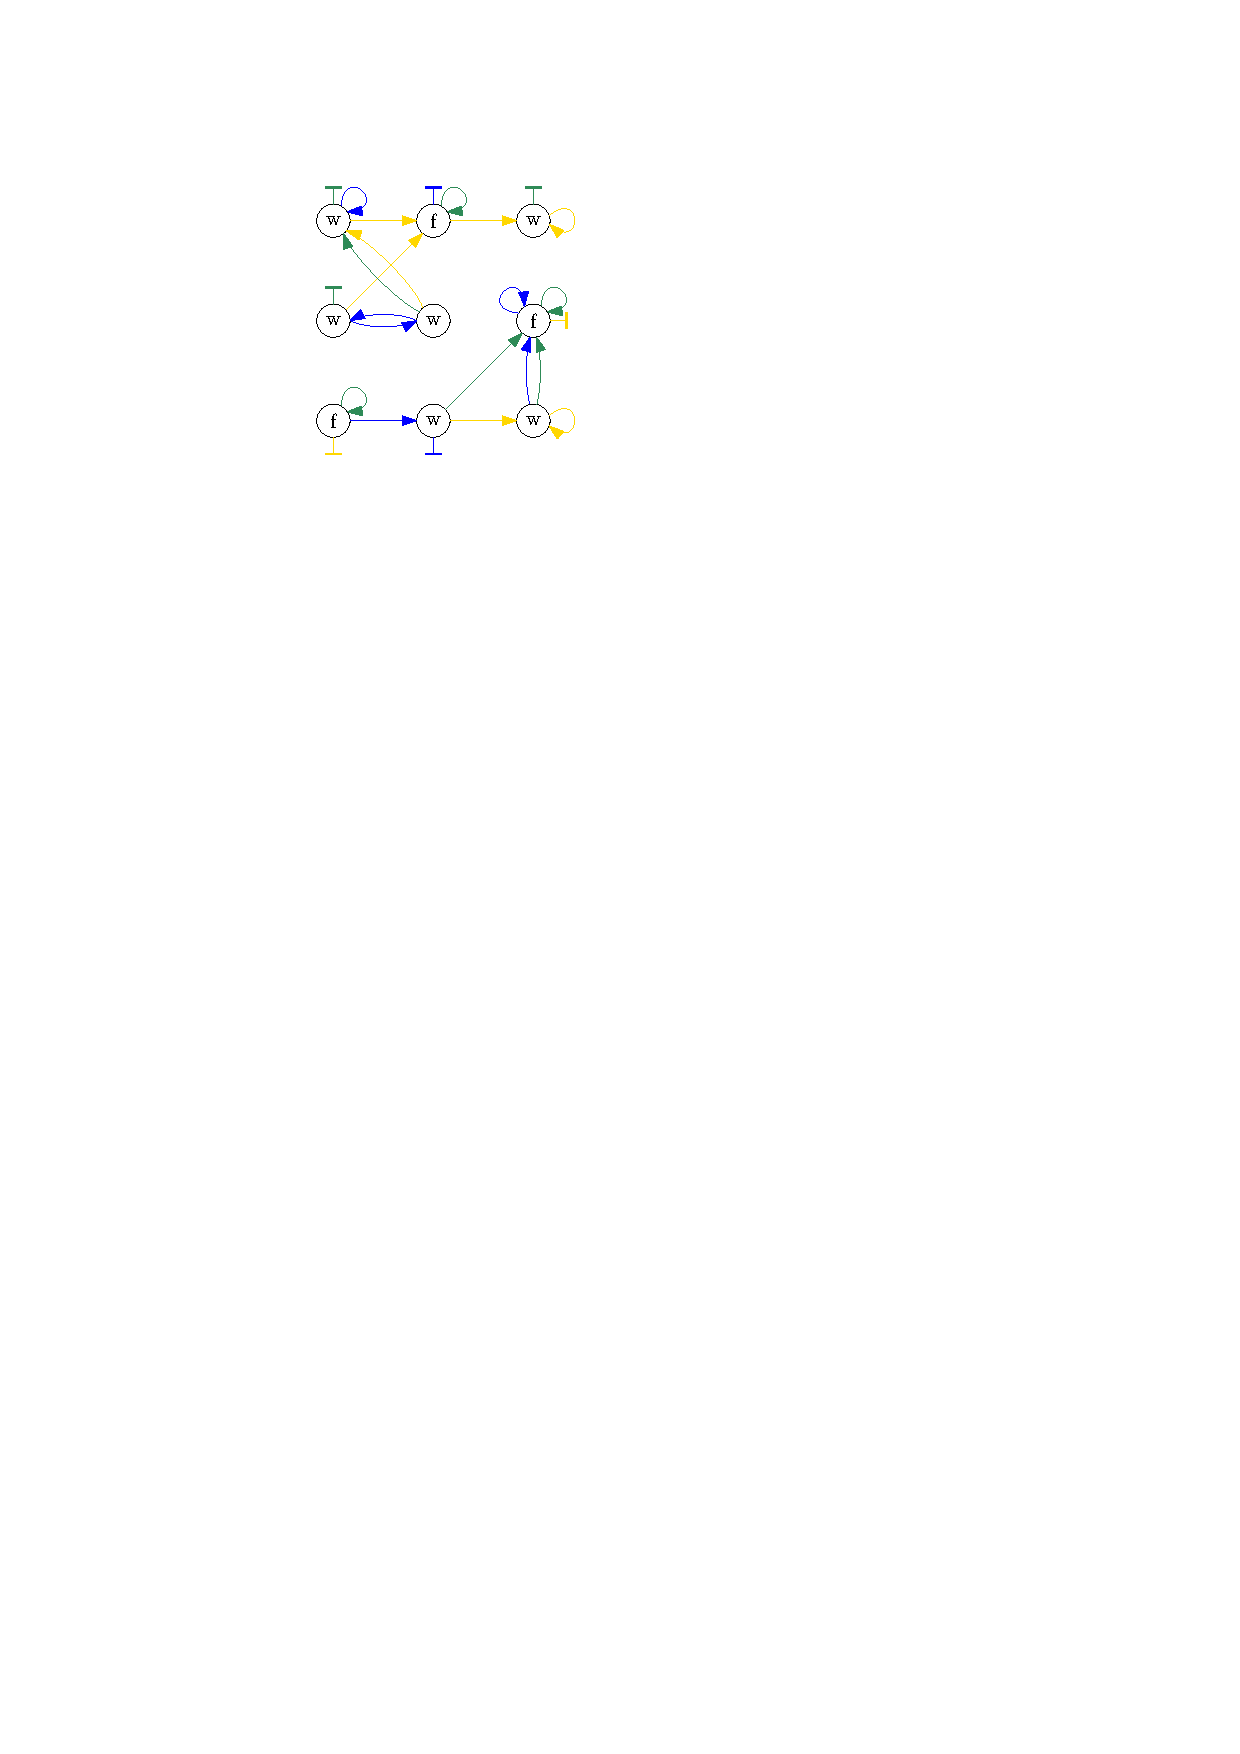
\includegraphics[page=1,width=.4\textwidth]{img/f-combined}
    \caption{Visualisierung der Funktionsverkettung durch $F$}
\end{figure}



\subsubsection{Wie muss ein Fixpunkt aussehen?}

\begin{enumerate}
    \item Für alle Zustände mit Wahrheitswert $\false$ muss der Fixpunkt eine Schleife ($\id$) liefern.
        \begin{figure}[H]
            \centering
            \includegraphics[page=2,width=.15\textwidth]{img/f-combined}
        \end{figure}
    \item Es gibt Zustände mit Wahrheitswert $\true$, die nach endlich vielen Schritten mit $\mathcal{S}$ (gelb) einen Zustand mit Wahrheitswert $\false$ erreichen.
        \begin{figure}[H]
            \centering
            \includegraphics[page=3,width=.6\textwidth]{img/f-combined}
        \end{figure}
    \item Es gibt Zustände mit Wahrheitswert $\true$, die nicht nach endliche vielen Schritten einen Zustand mit Wahrheitswert $\false$ erreichen.
        \begin{enumerate}
            \item $w \to w \to w \to \dots$
\begin{lstlisting}[language=Pascal]
x := 1;
while true do
    x := x + 1
\end{lstlisting}
                \begin{figure}[H]
                    \centering
                    \includegraphics[page=4,width=.6\textwidth]{img/f-combined}
                \end{figure}
                Hier müssen alle Pfeile zum selben Zustand zeigen, egal welcher genau das ist.
            \item  $w_1 \to w_2 \to w_2 \to w_1$
\begin{lstlisting}[language=Pascal]
x := 0;
while x != -1 do
    x := (x + 1) mod 10
\end{lstlisting}
                \begin{figure}[H]
                    \centering
                    \includegraphics[page=5,width=.22\textwidth]{img/f-combined}
                \end{figure}
                Hier müssen ebenfalls alle Pfeile zum selben Zustand zeigen, egal welcher genau das ist.
            \item $w \to w \to w \to \bot$
\begin{lstlisting}[language=Pascal]
x := 1;
while x < 20 do
    x := x + 1;
    if x = 10 then
        while true do skip
    else
        ...
\end{lstlisting}
        \begin{figure}[H]
            \centering
            \includegraphics[page=6,width=.6\textwidth]{img/f-combined}
        \end{figure}
        \end{enumerate}
        Für die Fälle (a) und (b) ist der Fixpunkt also fix aber beliebig (inklusive $\bot$).
\end{enumerate}

\par\bigskip
Das Ergebnis unserer informellen Überlegung ist:
\begin{itemize}
    \item Wir erwarten, dass \emph{immer ein Fixpunkt existiert}.
    \item Ein solcher Fixpunkt ist nicht immer eindeutig. Für Zustände, bei denen die \texttt{while}-Schleife nicht terminiert, kann es ggf. mehrere Möglichkeiten für einen Fixpunkt geben.

        In diesem Fall hätten wir gern den Fixpunkt, der $\bot$ für nicht-terminierende Schleifen liefert.
\end{itemize}


\subsubsection{Fixpunktiteration}

\begin{remark}[Idee]
    Finde die richtigen Fixpunkt durch Fixpunktiteration. Starte mit der Zustandsüberführungsfunktion \[
    f_{\bot} : f_{\bot}(\sigma) = \bot \quad \forall \sigma \in \State
    \]
    welche $F$ wiederholt auf $f_{\bot}$ an, schaue was passiert.

    $\Rightarrow$ Der ``Grenzwert'' ist der gewünschte Fixpunkt.

    Z.\,B. bei (c.a) und (c.b) bleibt die Funktion nach wiederholter Anwendung überall $\bot$.
\end{remark}

\begin{definition}[Fixpunktoperator]
    \begin{align*}
        f_0 & = f_{\bot} \\
        f_n &= F(f_{n-1}) \quad n \geq 1 \\
        \fix(f) & := \lim_{n \to \infty} f_n
    \end{align*}

    Aber wie ist der Grenzwert in diesem Kontext definiert?
\end{definition}



\subsection{Relationen und Ordnungen}

\begin{definition}
    Sei $\mathcal{F} = \{ f \;\vert\; f: \State \to \State \}$ die Menge aller \emph{partiellen} Zustandsüberführungsfunktionen. Wir definieren auf $\mathcal{F}$ eine Relation $\sqsubseteq$ durch \[
        f \sqsubseteq g :\Longleftrightarrow \forall \sigma, \sigma' \in \State: f(\sigma) = \sigma' \Rightarrow g(\sigma) = \sigma'
        \]
        \dh{} überall, wo $f$ definiert ist, ist auch $g$ definiert und liefert denselben Wert.
\end{definition}

\par\medskip
\begin{example}
    $g_1, g_2, g_3, g_4 : \State \to \State$
    \begin{align*}
        g_1(\sigma) & = \sigma \quad \forall \sigma \in \State \\
        g_2(\sigma) & = \begin{cases}
            \sigma & \text{falls } \sigma(x) \geq 0 \\
            \bot & \text{sonst} \\
        \end{cases} \\
        g_3(\sigma) & = \begin{cases}
            \sigma & \text{falls } \sigma(x) \leq 0 \\
            \bot & \text{sonst} \\
        \end{cases} \\
        g_4(\sigma) & = \begin{cases}
            \sigma & \text{falls } \sigma(x) = 0 \\
            \bot & \text{sonst} \\
        \end{cases} \\
    \end{align*}
    Behauptung:
    \begin{align*}
        g_4 \sqsubseteq g_2 \sqsubseteq g_1 \\
        g_4 \sqsubseteq g_3 \sqsubseteq g_1 \\
        g_4 \sqsubseteq g_1 \tag{*}
    \end{align*}
    $(*)$ folgt aus Transivität da die Relation eine Ordnungsrelation ist, aber das haben wir noch nicht bewiesen.

    Jedoch sind $g_2$ und $g_3$ nicht vergleichbar.
\end{example}

\par\bigskip
\begin{remark}[Fakt]
    $\sqsubseteq$ ist eine Ordnungsrelation auf $\mathcal{F}$. Das bedeutet, sie ist
    \begin{itemize}
        \item reflexiv: $f \sqsubseteq f$
        \item transitiv: $f \sqsubseteq g \wedge g \sqsubseteq h \Rightarrow f \sqsubseteq h$
        \item antisymmetrisch: $f \sqsubseteq g \wedge g \sqsubseteq f \Rightarrow f = g$
    \end{itemize}

    $(\mathcal{F}, \sqsubseteq)$ ist eine \emph{Halbordnung} (poset bzw. partially ordered set).
\end{remark}

\par\medskip
\begin{definition}
    Ein Element $f \in \mathcal{F}$ heißt \emph{Minimum}, falls für alle $g \in \mathcal{F}$ gilt \[
    f \sqsubseteq g
    \]
\end{definition}

\begin{observations}
    Im Allgemeinen, muss es kein Minimum in einem poset geben (\zb{} unendliche Ordnung oder mehrere nicht vergleichbare minimale Elemente). Wenn ein \emph{Minimum} existiert, dann ist es \emph{eindeutig} (wegen Antisymmetrie).

    Aber $(\mathcal{F}, \sqsubseteq)$ hat ein Minimum und zwar $f_{\bot}$.
\end{observations}



%%%%%%%%%%%%%%%%%%%%%%%%%%%%%%%%%%%%%%%%%%%%%%%%%%%%%%%%%%%%%%%%%%%%%
\newpage
\hfill 08.07.
%%%%%%%%%%%%%%%%%%%%%%%%%%%%%%%%%%%%%%%%%%%%%%%%%%%%%%%%%%%%%%%%%%%%%

\begin{remark}[Ziel für den Rest der Vorlesung]
    Konvergenz der Fixpunktiteration beweisen.
\end{remark}

\begin{definition}[Obere Schranke, Supremum]
    Sei $\mathcal{G} \subseteq \mathcal{F}$, dann ist auch $(\mathcal{G}, \sqsubseteq)$ eine Halbordnung.

    Ein Element $f \in \mathcal{F}$ heißt \emph{obere Schranke} von $\mathcal{G}$, falls \[
        \forall g \in \mathcal{G}: g \sqsubseteq f
    \]

    Eine obere Schranke von $\mathcal{G}$ heißt \emph{Supremum} ``$\sup \mathcal{G}$'', falls für alle oberen Schranken $f'$ von $\mathcal{G}$ gilt $f \sqsubseteq f'$ \dh{} es ist die kleinste obere Schranke.

    Falls ein \emph{Supremum} existiert, so ist es \emph{eindeutig}. Falls die obere Schranke innerhalb von $\mathcal{G}$ liegt, so ist sie auch das Maximum und Supremum von $\mathcal{G}$.
\end{definition}

\par\bigskip
\begin{definition}
    Sei $\mathcal{G} \subseteq \mathcal{F}$. Wir nennen $\mathcal{G}$ eine \emph{Kette} (chain), falls $\mathcal{G}$ total geordnet ist, \dh{} \[
        \forall g_1, g_2 \in \mathcal{G}: g1 \sqsubseteq g_2 \vee g_2 \sqsubseteq g_1
    \]
\end{definition}

\begin{example}
    Folgende Beispiele sind Ketten:
    \begin{itemize}
        \item Die leere Menge $\varnothing \subseteq \mathcal{F}$ ist eine Kette.
        \item Jede 1-elementige Menge ist eine Kette.
        \item Sei $x \in \Var$ eine Variable. Für $n \in \mathbb{N}$ definiere wir $g_n \in \mathcal{F}$ durch \begin{align*}
                g_n: & \State \to \State \\
                g_n(\sigma) & = \begin{cases}
                    \bot & \text{falls } \sigma(x) > n \\
                    \sigma[x \mapsto -1] & \text{falls } \sigma(x) \in \{ 0, \dots, n \} \\
                    \sigma & \text{falls } \sigma(x) < 0
                \end{cases}
            \end{align*}
            Die Menge $\{ g_n \mid n \in \mathbb{N} \}$ ist eine Kette in $(\mathcal{F}, \sqsubseteq)$, denn es gilt \[
                    g_n \sqsubseteq g_m \Leftrightarrow n \leq m
                \]
\begin{lstlisting}[escapeinside={/*}{*/}, language=Pascal, caption=Snippet für $g_n$]
while x >= 0 do  /*\label{code:loopdec}*/
    x := x - 1
\end{lstlisting}
            % TODO: foto
            \emph{Ziel:} Die Funktion \begin{align*}
                g_{\infty}: & \State \to \State \\
                g_{\infty} & = \begin{cases}
                    \sigma[x \mapsto -1] & \text{falls } \sigma(x) \geq 0 \\
                    \sigma & \text{sonst}
                \end{cases}
            \end{align*}
            ist die Semantik von Listing~\ref{code:loopdec}.

            Nun sehen wir, dass \[
                g_{\infty} = \sup \{ g_n \mid n \in \mathbb{N} \}
            \]
    \end{itemize}
\end{example}

\par\bigskip
\begin{definition}[Kettenvollständigkeit]
    Eine Halbordnung heißt \emph{kettenvollständig} (ccpo: chain-complete-partial order), falls jede Kette ein Supremum besitzt.
\end{definition}

\par\medskip
\begin{example}
    $(\mathbb{N}, \leq)$ ist nicht kettenvollständig. Die Menge der geraden Zahlen $\{ 2, 4, \dots \}$ ist eine Kette ohne Supremum.

    \par\medskip
    $(\mathcal{P}(\{ 1, 2, 3 \}), \subseteq)$ ist kettenvollständig.
    \begin{figure}[H]
        \centering
        % https://tex.stackexchange.com/questions/584458/drawing-a-hasse-diagram-in-latex
        \begin{tikzcd}[row sep=1.5cm, column sep=1.7cm]
                             & \{1,2,3\} \\
            \{1,2\}\urar       & \{1,3\}\uar \arrow[from=dr]                        & \{2,3\}\ular \\
            \{1\}\uar\urar & \{2\}\ular[crossing over] \urar[crossing over] & \{3\}\uar\\
                             & \varnothing \ular\uar\urar
        \end{tikzcd}
        \caption{Hasse-Diagramm für $(\mathcal{P}(\{1,2,3\}), \subseteq)$}
    \end{figure}

    \par\medskip
    $(\mathcal{P}(\mathbb{N}), \subseteq)$ ist auch kettenvollständig. Sei $X \in (\mathcal{P}(\mathbb{N}), \subseteq)$ eine Kette, also eine Menge von Teilmengen von $\mathbb{N}$, sodass $\forall A, B \in X: A \subseteq B \vee B \subseteq A$.\\
    Es ist $\sup X = \bigcup_{A \in X} A = Z$, da \begin{enumerate}
        \item Sei $A = X$. Dann ist $A \subseteq Z$.
        \item $Z$ ist kleinste obere Schranke. Sei $Y$ obere Schranke von $X$.

            Zu zeigen: $Z \subseteq Y$.

            Nimm $z \in Z$, zeige, dass $z \in Y$.
            \begin{align*}
                z \in Z \Rightarrow \exists A \subseteq Z \text{ mit } z \in A
            \end{align*}
            Da $Y$ obere Schranke von $X$ ist und $a \in X$, muss $A \subseteq Y$. Also folgt, $z \in Y$.
    \end{enumerate}
\end{example}

\par\bigskip
\begin{remark}[Fakt]
    Sei $(\mathcal{D}, \sqsubseteq)$ ccpo. Dann besitzt $\mathcal{D}$ ein Minimum, nämlich \[
            d_{\bot} = \sup \varnothing
        \]
\end{remark}

\begin{proof}
    Sei $d_{\bot} = \sup \varnothing$. $d_{\bot}$ existiert nach Annahme. Und sei $d \in \mathcal{D}$. Nach Definition ist $d$ eine obere Schranke von $\varnothing$. Da $d_{\bot} = \sup \varnothing$, muss $d_{\bot} \sqsubseteq d$ sein, \dh{} $d_{\bot}$ ist Minimum.
\end{proof}

\par\bigskip
\begin{theorem} \label{theorem:fkette}
    $(\mathcal{F}, \sqsubseteq)$ ist kettenvollständig.

    Sei $\mathcal{G} \subseteq \mathcal{F}$ eine Kette. Dann ist $\sup \mathcal{G}$ die Funktion mit \[
        \graph(\sup \mathcal{G}) = \bigcup \, \{ \graph(g) \mid g \in \mathcal{G} \}
    \]
    \dh{} \[
        (\sup \mathcal{G})(\sigma) = \sigma' \Leftrightarrow \exists g \in \mathcal{G}: g(\sigma) = \sigma'
    \]
\end{theorem}

\begin{proof}
    Wir müssen die folgenden Eigenschaften beweisen:
    \begin{enumerate}
        \item Wohldefiniertheit

            Seien $g_1, g_2 \in \mathcal{G}$ und sei $\sigma \in \State$, sodass $g_1(\sigma) \neq \bot \neq g_2(\sigma)$. Da $\mathcal{G}$ eine Kette ist, muss gelten $g_1 \sqsubseteq g_2 \vee g_2 \sqsubseteq g_1$. In beiden Fällen folgt $g_1(\sigma) = g_2(\sigma)$. Also ist der Wert von $(\sup \mathcal{G})(\sigma)$ wohldefiniert.
        \item obere Schranke

            Aus der Definition folgt direkt, dass $(\sup \mathcal{G})$ eine obere Schrank ist: \[
                g \in \mathcal{G}, \; \sigma, \sigma' \in \State, \; g(\sigma) = \sigma' \implies (\sup \mathcal{G})(\sigma) = \sigma'
            \]
        \item kleinste obere Schranke

            $(\sup \mathcal{G})$ ist obere Schranke. Sei $h$ eine obere Schranke.

            Zu zeigen: $(\sup \mathcal{G}) \sqsubseteq h$.

            Sei $\sigma, \sigma' \in \State$. $(\sup \mathcal{G})(\sigma) = \sigma'$, \dh{} $\exists g \in \mathcal{G}: g(\sigma) = \sigma'$, \dh{} $h$ ist obere Schranke, \dh{} $g \sqsubseteq h$, also muss $h(\sigma) = \sigma'$.
    \end{enumerate}
\end{proof}

Idee der Fixpunktiteration: \begin{align*}
    f_0 & = f_{\bot} \\
    f_1 & = F(f_0) \\
    \vdots \\
    f_{\infty} & = \sup \, \{ f_n \mid n \in \mathbb{N} \}
\end{align*}
Dann soll gelten: $f_{\infty} = F(f_{\infty})$.

Wenn also gelten würde \[
    F\left(\lim_{n \to \infty} f_n\right) = \lim_{n \to \infty} F(f_n)
\] wären wir fertig. Das ist die \emph{Stetigkeit}.



%%%%%%%%%%%%%%%%%%%%%%%%%%%%%%%%%%%%%%%%%%%%%%%%%%%%%%%%%%%%%%%%%%%%%
\newpage
\hfill 15.07.
%%%%%%%%%%%%%%%%%%%%%%%%%%%%%%%%%%%%%%%%%%%%%%%%%%%%%%%%%%%%%%%%%%%%%

\begin{remark}[Letztes Mal]
    Satz~\ref{theorem:fkette}: $(\mathcal{F}, \sqsubseteq)$ ist kettenvollständig.

    Was bisher fehlt ist ein in Konzept von Stetigkeit, sodass man Folgendes schreiben kann: \[
        \lim_{n \to \infty} f(x_n) = f\left(\lim_{n \to \infty} x_n\right)
    \]
\end{remark}


\par\medskip
\begin{definition}[Monotonie]
    Eine totale Funktion $f: D \to Z$ heißt \emph{monoton}, falls für alle $d_1, d_2 \in D$ gilt \[
        d_1 \sqsubseteq d_2 \Rightarrow f(d_1) \sqsubseteq' f(d_2)
    \]
\end{definition}

\begin{observations}
    Wir beobachten folgende Eigenschaften:
    \begin{enumerate}
        \item Seien $(\mathcal{D}, \sqsubseteq), (\mathcal{D}',\sqsubseteq'), (\mathcal{D}'',\sqsubseteq'')$ ccpos und $f_1: \mathcal{D} \to \mathcal{D}'$ und $f_2: \mathcal{D}' \to \mathcal{D}''$ monoton Funktionen.

            Dann ist auch $f_1 \circ f_2$ monoton.
        \item Seien $(\mathcal{D}, \sqsubseteq), (\mathcal{D}',\sqsubseteq')$ ccpos und $f: \mathcal{D} \to \mathcal{D}'$ eine monoton Funktion. Sei $\mathcal{K}$ eine Kette. Dann ist $f(\mathcal{K})$ eine Kette in $\mathcal{D}'$. Wenn $\mathcal{D}$ endlich ist, dann ist das Supremum von $\mathcal{D}'$: \[
                \sup' \mathcal{D}' = f(\sup \mathcal{D})
            \]

            Im Allgemeinen gilt: $f(\sup S) \sqsubsetneqq' \sup' f(S)$
    \end{enumerate}
\end{observations}


\par\bigskip
\begin{definition}[Stetigkeit]
    Seien $(\mathcal{D}, \sqsubseteq), (\mathcal{D}',\sqsubseteq')$ ccpos und $f: \mathcal{D} \to \mathcal{D}'$ heißt \emph{stetig} wenn:
    \begin{enumerate}
        \item $f$ ist monoton.
        \item Für alle nichtleeren Ketten $\mathcal{S} \in \mathcal{D}$ gilt $\sup' f(\mathcal{S}) = f(\sup\, \mathcal{S})$.
    \end{enumerate}
\end{definition}

\par\medskip
\begin{observation}
    Seien $(\mathcal{D}, \sqsubseteq), (\mathcal{D}',\sqsubseteq'), (\mathcal{D}'',\sqsubseteq'')$ ccpos und seien die beiden Funktionen $f: \mathcal{D} \to \mathcal{D}'$ und $f': \mathcal{D}' \to \mathcal{D}''$ stetig.

    Dann ist $f' \circ f: \mathcal{D} \to \mathcal{D}''$ stetig.
\end{observation}


\par\bigskip
\begin{theorem}
    Sei $(\mathcal{D}, \sqsubseteq)$ ccpo mit Minimum $d_h$ und sei $F : \mathcal{D} \to \mathcal{D}$ eine stetige Funktion. Setze $f_0 = d_{\bot}$ und $f_n = f(f_{n-1})$.

    \begin{enumerate}
        \item Dann ist $\{ f_n \mid n \in \mathbb{N} \}$ eine Kette.
        \item Sei $\fix(F) = \sup \{ f_n \mid n \in \mathbb{N} \}$. Dann gilt $F(\fix(F)) = \fix(F)$.
        \item Außerdem gilt $\forall g \in \mathcal{D}, F(g) = g: g \geq \fix(F)$.
    \end{enumerate}
\end{theorem}

\begin{proof}
    Wir führen den Beweis stückweise.
    \begin{enumerate}
        \item $\{ f_n \mid n \in \mathbb{N} \}$ ist eine Kette. \\
            Seien $f_n, f_m$ mit $m > n$. Zu zeigen $f_n \sqsubseteq f_m$.

            Setze $a = n - m > 0$. Da $f_0 = d_{\bot}$ Minimum ist, gilt $f_0 \sqsubseteq f_a$. Da $F$ stetig ist, folgt
            \begin{align*}
                F(f_0) & \sqsubseteq F(f_n) \\
                \Rightarrow f_1 & \sqsubseteq f_{a+1} \\
                & n\text{-mal} \dots \\
                \Rightarrow f_n & \sqsubseteq f_{a+n}
            \end{align*}

        \item $\fix(F)$ ist Fixpunkt von $F$.
            \begin{align*}
                F(\fix(F)) & = F(\sup \{f_n \mid n \in \mathbb{N} \}) \tag{Def} \\
                & = \sup F(\{f_n \mid n \in \mathbb{N} \}) \tag{Stetigkeit} \\
                & = \sup \{F(f_n) \mid n \in \mathbb{N} \} \\
                & = \sup \{f_{n+1} \mid n \in \mathbb{N} \} \tag{Def} \\
                & = \sup (\{f_{n+1} \mid n \in \mathbb{N} \} \cup \{ d_{\bot} \}) \tag{Minimum} \\
                & = \fix(F) \tag{Def}
            \end{align*}

        \item $\fix(f)$ ist minimaler Fixpunkt.

            Sei $g \in \mathcal{D}$ und $F(g) = g$. Es gilt $g \sqsupseteq d_{\bot}$ ($d_{\bot}$ ist Minimum).

            Also auch $F(g) \sqsupseteq F(d_{\bot})$ bzw. $g \sqsupseteq f_1$. Also auch $F(g) \sqsupseteq F(f_1)$ bzw. $g \sqsupseteq f_2$ usw.

            Also gilt nach Induktion $g \sqsupseteq f_n, n \in \mathbb{N}$. $g$ ist eine obere Schranke von $\{f_n \mid n \in \mathbb{N} \}$. Nach Defintion vom Supremum, ist $g$ die kleinste obere Schranke.
            \[ \fix(f) = \sup \{ f_n \mid n \in \mathbb{N} \} \sqsubseteq g \]
    \end{enumerate}
\end{proof}

\par\medskip
\emph{Zurück zum ursprünglichem Ziel:} Nun möchten wir schreiben: \[ \Sdssem{\texttt{while $b$ do $S$}} = \fix(F)
\] wobei $F(g) = \cond(\Bsem{b}, g \circ \Sdssem{S}, \id)$ und $f \circ g: \State \to \State$.


Nach dem Satz müssen wir jetzt nur noch überprüfen, dass $F$ stetig ist.
Das funktioniert so: Wir beobachten, dass sich $F$ schreiben lässt als $F = F_2 \circ F_1$, wobei $F_1(g) = g \circ \Sdssem{S}$
und $F_2(g) = \cond(\Bsem{b}, g, \id)$.

$\Sdssem{\cdot}$ ist schwierig, also beweisen wir die Stetigkeit getrennt.

\begin{proof}[Skizze]
    Zu zeigen:
    \begin{enumerate}
        \item $F_2$ ist stetig, durch detaillierte Analyse.
        \item $F_1$ ist stetig. Beobachtung: Für jedes feste $g_0: \State \to \State$:

            Ist $F_1(f) = f \circ g_0$ stetig?
    \end{enumerate}
    $\Rightarrow F_2 \circ F_1$ ist stetig.
\end{proof}


\begin{theorem}
    $\Sdssem{\cdot}$ definiert eine semantische Funktion auf der Menge aller \texttt{while}-Programme.
\end{theorem}

\begin{proof}[Skizze]
    Durch strukturelle Induktion nach der Anweisung $S$.
\end{proof}



\subsection{Eigenschaften der denotatiollen Semantik}

Seien $S_1, S_2$ Anweisungen. Wir sagen, sie sind semantisch äquivalent, wenn \[
    \Sdssem{S_1} = \Sdssem{S_2}
\] (Vergleich als mathematische Funktionen).

\par\medskip
\begin{example}
    $S$ und $S; \texttt{skip}$ sind semantisch äquivalent.

    \begin{align*}
        \Sdssem{S_1} & = \Sdssem{S_1; \texttt{skip}} \\
        & =\Sdssem{\texttt{skip}} \circ \Sdssem{S_1} \\
        & = \id \circ \; \Sdssem{S_1} \\
        & = \Sdssem{S_1} \quad \checkmark
    \end{align*}

    oder auch \[
        S_1; (S_2; S_3) \text{ und } (S_1; S_2); S_3
    \] durch Assoziositivität der Funktionskompositon. Und auch \[
        \texttt{while $b$ do $S$} \text{ und } \texttt{if $b$ then ($S$; while $b$ do $S$) else skip}
    \]
\end{example}


\begin{theorem}
    Sei $S$ eine Anweisung in der \texttt{while}-Sprache, dann gilt: \[
        \Sdssem{S} = \Ssossem{S}
    \]
\end{theorem}

\begin{proof}[Skizze]
    Durch Fallunterscheidung/Induktion.

    Der Beweis verwendet die Antisymmetrie von $(\mathcal{F}, \sqsubseteq)$. Wir zeigen, dass \[
        \Sdssem{\cdot} \sqsubseteq \Ssossem{\cdot} \text{ und } \Ssossem{\cdot} \sqsubseteq \Sdssem{\cdot}
    \]

    \begin{enumerate}
        \item $\Ssossem{\cdot} \sqsubseteq \Sdssem{\cdot}$ \\
            Sei $S$ eine Anweisung, dann gilt $\Ssossem{\cdot} \sqsubseteq \Sdssem{\cdot}$, \dh{} für alle $\sigma, \sigma'$ gilt:
            Falls $\Ssossem{s}(\sigma) = \sigma'$, dann auch $\Sdssem{s}(\sigma) = \sigma'$.

            Nach Definition gilt \[
                \Ssossem{S}(\sigma) = \sigma' \Longleftrightarrow \langle S, \sigma \rangle \Rightarrow^* \sigma
            \]
            Dann zeigen wir: Wenn $\langle S, \sigma \rangle = \sigma'$, dann gilt $\Sdssem{S}(\sigma)=\sigma'$.
            Und wenn gilt $\langle S, \sigma \rangle = \langle S', \sigma' \rangle$, dann gilt $\Sdssem{S}(\sigma) = \Sdssem{S'}(\sigma')$.

        \item $\Sdssem{\cdot} \sqsubseteq \Ssossem{\cdot}$ \\

            Sei $S$ eine Anweisung, dann gilt $\Sdssem{\cdot} \sqsubseteq \Ssossem{\cdot}$. Also gilt \[
                    \Sdssem{S}(\sigma) = \sigma' \implies \Ssossem{S}(\sigma) \Rightarrow^* \sigma'
            \]
            Beweis: Strukturelle Induktion und Definition des Fixpunktoperators (Beweis ist lang).
    \end{enumerate}
\end{proof}



%%%%%%%%%%%%%%%%%%%%%%%%%%%%%%%%%%%%%%%%%%%%%%%%%%%%%%%%%%%%%%%%%%%%%
\newpage
\hfill 22.07.
%%%%%%%%%%%%%%%%%%%%%%%%%%%%%%%%%%%%%%%%%%%%%%%%%%%%%%%%%%%%%%%%%%%%%

\subsection{Programmanalyse mit denotationeller Semantik}

\emph{Ziel:} Erhalte Informationen über das \emph{dynamische} Verhalten eines Programms durch eine \emph{statische} Analyse ohne das Programm auszuführen, \zb{} mit \texttt{lint} für die Sprache C.

\begin{example}
    Verschiedene Anwendungen für statische Programmanalyse:
    \begin{itemize}
        \item definition-use-Analyse: Sind Variablen initialisiert bevor sie benutzt werden?
        \item constant-propagation: Werte/Ausdrücke, im Vorhinein auswerten, die nicht vom Zustand des Programms abhängen.
        \item Intervall-Analyse: Bestimme Intervalle für mögliche Variablenwerte.
    \end{itemize}

\end{example}

\emph{Hier:} Sonderfall der Intervall-Analyse: \emph{Vorzeichenanalyse}, \dh{} bestimme statisch mögliche Vorzeichen für die Variablen im Programm.



\subsubsection{Vorzeichenanalyse}

\emph{Idee:} Arbeite mit Funktionen, die Eigenschaften von Zuständen abbilden und nicht die Zustände selbst (\emph{property states}). Dazu benötigen wir die Menge abstrakter Eigenschaften von Programmvariablen $\mathcal{P}$.

\par\medskip
\begin{definition} \label{def:vorzeichenanalyse}
    \[
    \mathcal{P} = \{ \text{POS}, \text{NEG}, \text{NULL}, \text{BEL} \}
    \]
    wobei BEL ``beliebig'' bedeutet.

    Wir definieren außerdem eine partielle Ordnung $\sqsubseteq_{\mathcal{P}}$ auf $\mathcal{P}$ mit der Bedeutung ``$p_1 \sqsubseteq_{\mathcal{P}} p_2$'': $p_1$ ist mindestens so spezifisch wie $p_2$, \zb{} POS $\sqsubseteq_{\mathcal{P}}$ BEL.

    Wir nehmen an, dass $\sqsubseteq_{\mathcal{P}}$ so definiert ist, dass alle Teilmengen $Y \subseteq \mathcal{P}$ ein Supremum besitzen (\emph{vollständiger Verband}). Dann gibt das Supremum die allgemeinste Eigenschaft einer Menge von Eigenschaften an.
\end{definition}

In der Programmanalyse arbeiten wir mit \emph{abstrakten Zustandseigenschaften} (property states), die jeder Variable eine Eigenschaft zuordnen statt eines konkreten Wertes: \[
    \PState: \Var \to \mathcal{P}
\]

\begin{lemma}
    Wenn $\mathcal{P}$ ein vollständiger Verband ist (siehe \defref{def:vorzeichenanalyse}), dann gilt das auch für $\PState$.

    Genaue Formulierung nicht hier \dots
\end{lemma}

\par\bigskip
\emph{Idee:} Bisher hatten wir $\mathcal{S} : \Stm \to (\State \to \State)$. Nun bentrachten wir die Analysefunktion $\mathcal{DS}: \Stm \to (\PState \to \PState)$.

\begin{remark}[Halteproblem]
    Wir können nicht erwarten, dass die Programmanalyse immer die genauest mögliche Antwort liefert.

\begin{lstlisting}[language=Pascal]
y := 1;
if bla then
    x := 1;
else
    S;
    x := -1;
y := x
\end{lstlisting}

    Hier hängt die Vorzeichenanalyse für $y$ davon ab, ob $S$ terminiert oder nicht, \dh{} unsere Analyse ist notwendigerweise approximativ und wird sagen, dass $y$ negativ sein könnte.
\end{remark}



\subsubsection{Vorzeichenanalyse von \texttt{while}}

\begin{enumerate}
    \item Wir definieren die gewünschte Eigenschaft, \dh{} eine Variable ist entweder POS, NEG oder NULL.

        Füge zusätzliche Eigenschaften hinzu, um die Analyse detaillierter zu machen und einen vollständigen Verband zu erhalten: NONPOS, NONNEG, NONNULL, BEL und NONE (letzteres aus technischen Gründen, um für die leere Menge ein Supremum zu haben).

        Definiere Ordnung:
        \begin{figure}[H]
            \centering
            \begin{tikzcd}[row sep=1.5cm, column sep=1.7cm]
                                 & \text{BEL} \\
                \text{NONPOS}\urar       & \text{NONNULL}\uar \arrow[from=dr]                        & \text{NONNEG}\ular \\
                \text{NEG}\uar\urar & \text{NULL}\ular[crossing over] \urar[crossing over] & \text{POS}\uar\\
                                 & \text{NONE} \ular\uar\urar
            \end{tikzcd}
            \caption{Hasse-Diagramm für $(\mathcal{P}, \sqsubseteq_{\mathcal{P}})$ (oben allgemein, unten spezifisch)}
        \end{figure}

    \item Definiere property states: Definiere Verhältnis zwischen Zuständen und Zustandseigenschaften: \begin{align*}
            \abs_{\mathbb{Z}} & : \mathbb{Z} \to \mathcal{P} \\
            \abs_{\mathbb{Z}}(z) & = \begin{cases}
                \text{POS} & \text{falls } z > 0 \\
                \text{NULL} & \text{falls } z = 0 \\
                \text{NEG} & \text{falls } z < 0
            \end{cases}
        \end{align*}

        Dann ist $\PState: \Var \to \mathcal{P}$. Wir definieren \begin{align*}
            \abs & : \State \to \PState \\
            \big(\abs(\sigma)\big)(x) & = \abs_{\mathbb{Z}}(\sigma(x))
        \end{align*}

    \item Da die Wahrheitswerte im Programm vom Zustand abhängen, benötigen wir abstrakte Eigenschaften für die Wahrheitswerte, die aus den abstrakten Eigenschaften der Variablen folgen. \[
            \mathcal{T} = \{ \true, \false, \text{BEL}, \text{NONE} \}
        \]

        Wieder brauchen wir eine Ordnung:
        \begin{figure}[H]
            \centering
            \begin{tikzcd}[row sep=1cm, column sep=0.8cm]
                            & \text{BEL} \\
                \true\urar  &           & \false\ular \\
                            & \text{NONE} \ular\urar
            \end{tikzcd}
            \caption{Hasse-Diagramm für $\mathcal{T}$}
        \end{figure}

    \item Definiere \emph{Analysefunktion}: Analog zur semantischen Funktion, operiert aber auf Zustandseigenschaften anstelle von Zuständen: Für alle syntaktischen Kategorien definiere:

        \begin{enumerate}
            \item Arithmetische Ausdrücke \begin{align*}
                    \mathcal{DA} : \AExp \to (\PState & \to \mathcal{P}) \\
                    \mathcal{DA}\lsem z \rsem(\sigma) & = \abs_{\mathbb{Z}}(\mathcal{N}(z)) \\
                    \mathcal{DA}\lsem x \rsem(\sigma) & = \sigma(z) \\
                    \mathcal{DA}\lsem a_1 \square a_2 \rsem(\sigma) & = \mathcal{DA}\lsem a_1 \rsem(\sigma) \square_v \mathcal{DA}\lsem a_2 \rsem(\sigma) \tag{*} \\
                \end{align*}

                Hierbei (in (*)) simulieren $+_v$, $-_v$ und $\cdot_v$ das Verhalten des Vorzeichens \texttt{+}, \texttt{-} und \texttt{*}:
                \begin{align*}
                    \square_v : \mathcal{P} \times \mathcal{P} & \to \mathcal{P} \\
                    \text{\zb{}} \; \text{POS} +_v \text{POS} & = \text{POS} \\
                    \text{POS} +_v \text{NEG} & = \text{BEL} \\
                    \vdots
                \end{align*}

            \item Boolesche Ausdrücke \begin{align*}
                    \mathcal{DB} : \BExp \to (\PState & \to \mathcal{T}) \\
                    \mathcal{DB}\lsem\texttt{true}\rsem(\sigma) & = \true \\
                    \mathcal{DB}\lsem\texttt{false}\rsem(\sigma) & = \false \\
                    \mathcal{DB}\lsem a_1 \square a_2 \rsem(\sigma) & = \mathcal{DA}\lsem a_1 \rsem(\sigma) \square_v \mathcal{DA}\lsem a_2 \rsem(\sigma) \\
                    \mathcal{DB}\lsem \neg b \rsem(\sigma) & = \neg_{\tau} \mathcal{DB}\lsem b \rsem(\sigma) \\
                    \mathcal{DB}\lsem b_1 \square b_2 \rsem(\sigma) & = \mathcal{DB}\lsem b_1 \rsem(\sigma) \square_{\tau} \mathcal{DB}\lsem b_2 \rsem(\sigma)
                \end{align*}

            \item Anweisungen \begin{align*}
                    \mathcal{DS} : \Stm \to (\PState & \to \mathcal{P}) \\
                    \mathcal{DS}\lsem x \texttt{ := } a \rsem(\sigma) & = \sigma[x \mapsto \mathcal{DA}\lsem a \rsem(\sigma)] \\
                    \mathcal{DS}\lsem \texttt{skip} \rsem(\sigma) & = \sigma \\
                    \mathcal{DS}\lsem S_1 \texttt{; } S_2 \rsem(\sigma) & = \mathcal{DS}\lsem S_2 \rsem(\sigma) \circ \mathcal{DS}\lsem S_1 \rsem(\sigma) \\
                    \mathcal{DS}\lsem \texttt{if $b$ then $S_1$ else $S_2$} \rsem(\sigma) & = \cond_{\infty}(\mathcal{DB}\lsem b \rsem, \mathcal{DS}\lsem S_1 \rsem, \mathcal{DS}\lsem S_2 \rsem) \\
                    \mathcal{DS}\lsem \texttt{while $b$ do $S$} \rsem(\sigma) & = \fix(H) \\
                    H: h & \mapsto \cond_{\infty}(\mathcal{DB}(b), h \circ \mathcal{DS}(S), \id)
                \end{align*}

                mit \begin{align*}
                    \cond_{\infty}(f, h_1, h_2)(\sigma) & = \begin{cases}
                        \text{INIT} & \text{falls } f(\sigma) = \text{NONE} \\
                        h_1(\sigma) & \text{falls } f(\sigma) = \true \\
                        h_2(\sigma) & \text{falls } f(\sigma) = \false \\
                        \sup \{ h_1(\sigma), h_2(\sigma) \} & \text{falls } f(\sigma) = \text{BEL} \\
                    \end{cases}
                \end{align*}

                mit \begin{align*}
                    \text{INIT} & : \Var \to \mathcal{P} \\
                    \forall x \in \Var & : \text{INIT}(x) = \text{NONE}
                \end{align*}
        \end{enumerate}
\end{enumerate}



\end{document}
